\documentclass[10pt,letterpaper]{article}
\usepackage[top=0.85in,left=2.75in,footskip=0.75in]{geometry}

% amsmath and amssymb packages, useful for mathematical formulas and symbols
\usepackage{amsmath,amssymb}

% Use adjustwidth environment to exceed column width (see example table in text)
\usepackage{changepage}

% Use Unicode characters when possible
%\usepackage[utf8x]{inputenc}

% textcomp package and marvosym package for additional characters
\usepackage{textcomp,marvosym}


% Use nameref to cite supporting information files (see Supporting Information section for more info)
\usepackage{nameref,hyperref}

% line numbers
\usepackage[right]{lineno}

% ligatures disabled
\usepackage{microtype}
\DisableLigatures[f]{encoding = *, family = * }

% color can be used to apply background shading to table cells only
\usepackage[table]{xcolor}

% create "+" rule type for thick vertical lines
\newcolumntype{+}{!{\vrule width 2pt}}

% create \thickcline for thick horizontal lines of variable length
\newlength\savedwidth
\newcommand\thickcline[1]{%
  \noalign{\global\savedwidth\arrayrulewidth\global\arrayrulewidth 2pt}%
  \cline{#1}%
  \noalign{\vskip\arrayrulewidth}%
  \noalign{\global\arrayrulewidth\savedwidth}%
}

% \thickhline command for thick horizontal lines that span the table
\newcommand\thickhline{\noalign{\global\savedwidth\arrayrulewidth\global\arrayrulewidth 2pt}%@
\hline
\noalign{\global\arrayrulewidth\savedwidth}}


% Remove comment for double spacing
%\usepackage{setspace}
%\doublespacing

% Text layout
\raggedright
\setlength{\parindent}{0.5cm}
\textwidth 5.25in
\textheight 8.75in

% Bold the 'Figure #' in the caption and separate it from the title/caption with a period
% Captions will be left justified
\usepackage[aboveskip=1pt,labelfont=bf,labelsep=period,justification=raggedright,singlelinecheck=off]{caption}
\renewcommand{\figurename}{Fig}

% Use the PLoS provided BiBTeX style
%\bibliographystyle{plos2015}

% Header and Footer with logo
\usepackage{lastpage,fancyhdr,graphicx}
\usepackage{epstopdf}
\pagestyle{myheadings}
\pagestyle{fancy}
\fancyhf{}
\setlength{\headheight}{27.023pt}
\lhead{
\includegraphics[width=2.0in]{PLOS-submission.eps}}
\rfoot{\thepage/\pageref{LastPage}}
\renewcommand{\footrule}{\hrule height 2pt \vspace{2mm}}
\fancyheadoffset[L]{2.25in}
\fancyfootoffset[L]{2.25in}
\lfoot{\sf PLOS}

%% \documentclass{article} % For LaTeX2e
%% \usepackage{nips14submit_e,times}
%% \usepackage{hyperref}
\usepackage{url}
\usepackage[round]{natbib}
\usepackage{amsmath,amsfonts,amsthm}
\usepackage{mdframed}
\usepackage{bbm}
\usepackage{algorithm,algorithmic}
\usepackage{graphicx}
\usepackage{bm}
\usepackage{bbm}
\usepackage[titletoc]{appendix}
\usepackage{wrapfig}
\usepackage{afterpage}
\usepackage{amssymb}
\usepackage{booktabs}
\usepackage{ulem}
\usepackage{multirow}
% Remove brackets from numbering in List of References
\makeatletter
\renewcommand{\@biblabel}[1]{\quad#1.}
\makeatother

% Leave date blank
\date{}

% Header and Footer with logo
\usepackage{lastpage,fancyhdr,graphicx}
\usepackage{epstopdf}
\pagestyle{myheadings}
\pagestyle{fancy}
\fancyhf{}
\setlength{\headheight}{27.023pt}
\lhead{
\includegraphics[width=2.0in]{PLOS-submission.eps}}
\rfoot{\thepage/\pageref{LastPage}}
\renewcommand{\footrule}{\hrule height 2pt \vspace{2mm}}
\fancyheadoffset[L]{2.25in}
\fancyfootoffset[L]{2.25in}
\lfoot{\sf PLOS}

%% Include all macros below

\newcommand{\lorem}{{\bf LOREM}}
\newcommand{\ipsum}{{\bf IPSUM}}

\def\B#1{\bm{#1}}
%\def\B#1{\mathbf{#1}}
\def\trans{\mathsf{T}}

\newtheorem{theorem}{Theorem} \newtheorem{lemma}[theorem]{Lemma}
\newtheorem{proposition}[theorem]{Proposition}
\newtheorem{corollary}[theorem]{Corollary}
\newtheorem{definition}[theorem]{Definition}
\newtheorem*{definition*}{Definition}
\newtheorem{remark}{Remark}

%%%%%%%%%%%%%%%%%%%%%%%%%%%%%%%%%%%%%%%%%%%%%%%%%%%%%%%%%%%%%%%%%%%%%%%%%%%%%%%

\title{Dark Control:\\
       Towards a Unified Account of Default Mode Function\\
       by Markov Decision Processes}

\newcommand{\fix}{\marginpar{FIX}}
\newcommand{\new}{\marginpar{NEW}}
\DeclareMathOperator{\proj}{proj}
\DeclareMathOperator{\softmax}{softmax}
\DeclareMathOperator{\prox}{prox}
\DeclareMathOperator{\Prox}{Prox}
\DeclareMathOperator{\im}{im}

% some useful macros
\DeclareMathOperator{\dist}{dist} % The distance.
\DeclareMathOperator{\argmin}{argmin}
\DeclareMathOperator{\argmax}{argmax}
\DeclareMathOperator{\Id}{Id}
\DeclareMathOperator{\abs}{abs}
\newcommand{\R}{\mathbb{R}}
\newcommand{\N}{\mathbb{N}}
\newtheorem{thm}{Theorem}[section]
\newtheorem{prop}[thm]{Proposition}
\newtheorem{lem}[thm]{Lemma}
\newtheorem{cor}[thm]{Corollary}
\newtheorem{fact}[thm]{Fact}

\def\Id{\mathbf{I}}
\def\1{\mathbf{1}}
\def\X{\mathbf{X}}
\def\U{\mathbf{U}}
\def\V{\mathbf{V}}
\def\v{\mathbf{v}}
\def\u{\mathbf{u}}
\def\z{\mathbf{z}}
\def\Y{\mathbf{Y}}
\def\A{\mathbf{A}}
\def\B{\mathbf{B}}
\def\C{\mathbf{C}}
\def\N{\mathbf{N}}
\def\R{\mathbf{R}}
\def\Q{\mathbf{Q}}
\def\P{\mathbf{P}}
\def\W{\mathbf{W}}
\def\K{\mathbf{K}}
\def\a{\mathbf{a}}
\def\b{\mathbf{b}}
\def\s{\mathbf{s}}
\def\x{\mathbf{x}}

\newcommand{\suggestadd}[1]{{\color{blue} #1}}
\newcommand{\suggestremove}[1]{{\color{red} \sout{#1}}}

% \nipsfinalcopy % Uncomment for camera-ready version
%\nipsfinaltrue
%%%%%%%%%%%%%%%%%%%%%%%%%%%%%%%%%%%%%%%%%%%%%%%%%%%%%%%%%%%%%%%%%%%%%%%%%%%%%%%

\begin{document}

\author{Elvis Dohmatob\textsuperscript{1,2}, Guillaume Dumas\textsuperscript{4,5,6,7}, Danilo Bzdok\textsuperscript{1,2,3}
}

\maketitle
\small{
    \textbf{1} Universit\'e Paris-Saclay, INRIA, Parietal Team, Saclay, France\\
    \textbf{2} Universit\'e Paris-Saclay, CEA, Neurospin, Gif-sur-Yvette, France\\
    \textbf{3} Department of Psychiatry, Psychotherapy and Psychosomatics, RWTH Aachen University, Aachen, Germany\\
    \textbf{4} Institut Pasteur, Human Genetics and Cognitive Functions Unit, Paris, France\\
    \textbf{5} CNRS UMR 3571 Genes, Synapses and Cognition, Institut Pasteur, Paris, France\\
    \textbf{6} University Paris Diderot, Sorbonne Paris Cit\'e, Paris, France\\
    \textbf{7} Centre de Bioinformatique, Biostatistique et Biologie Int\'egrative, Paris, France
}

\begin{abstract}
The Default Mode Network (DMN) is believed to subserve the
baseline mental activity in humans.
%
Its highest energy consumption compared to other brain networks and
its intimate coupling with conscious awareness are both pointing to
an overarching function.
%
Many research streams support an evolutionarily adaptive role in
envisioning experience to anticipate the future.
In the present work, we propose a \textit{process model}
that tries to explain \textit{how}
the DMN may implement
continuous evaluation and prediction of the environment to guide behavior.
%
DMN function is recast in terms of
control theory and reinforcement learning by basing it on Markov decision processes.
%
We argue that our formal account of DMN function naturally accommodates as special cases
the previously proposed cognitive accounts on
(1) predictive coding,
(2) semantic associations, and
(3) a ``sentinel'' role.
%
Moreover, this process model for the neural optimization of complex behavior in the DMN
offers parsimonious explanations for
recent experimental findings in animals and humans.
\end{abstract}

% official NIPS keywords
\textbf{\\keywords}: mind-wandering, artificial intelligence, Markov decision processes

% autonomous learning systems
% \textbf{\\Get opinion from}: Danielle Bassett, Kai Vogeley, Mohammad Shakir,
% Guillaume Dumas, Smallwood, Tenenbaum

% \tableofcontents
% \listoffigures
% \listoftables

\section{Introduction}
%
In the absence of external stimulation, the human brain is not at rest.
In the beginning of the 21st century,
brain imaging may have been the first technique
to allow for the discovery of a unique brain network that would subserve
baseline mental activities
\citep{raichle2001pnas, randy2008, bzdok2015resting}.
The ``Default Mode Network'' (DMN) continues
to metabolize large quantities of
oxygen and glucose energy to maintain
neuronal computation
during free-ranging thought
\citep{kenet2003spontaneously, fiser2004small}.
The baseline energy demand is only weakly modulated
at the onset of defined psychological tasks \citep{raichle_baseline}.
At its opposite, during sleep, the
decoupling of brain structures discarded the idea of the DMN being
only a passive network resonance and rather supported an
important role in sustaining conscious awareness \citep{horovitz2009decoupling}.



This \textit{dark matter of brain physiology}
\citep{raichle2006brain} begs the question
of the biological purpose underlying DMN activity.
Despite observation of similar large-scale networks of co-varying spontaneous activity in MEG investigations \citep{de2010temporal,brookes2011investigating,baker2014fast}, the link between the fMRI BOLD signal and population-level neural activity is still unclear. If those frequency-specific electrophysiological correlations are proposed as complementary to those observed with BOLD \citep{hipp2015bold}, their role in DMN function remains challenging \citep{maldjian2014graph}.


What has early been described as the ``stream of consciousness''
in psychology \citep{james1890principles}
found a potential neurobiological manifestation
in the DMN
\citep{shul1997, raichle2001pnas}.
We propose that this set of some of the most advanced regions in
the association cortex \citep{mesulam1998sensation, margulies2016situating}
are responsible for higher-order control of human behavior.
Our functional account follows the notion of
``a hierarchy of brain systems with
the DMN at the top and the salience and dorsal attention systems
at intermediate levels, above thalamic and unimodal sensory
cortex'' \citep{carhart2010default}.



\subsection{Towards a formal account of default mode function: higher-order control of the organism}
The network nodes that compose the human DMN
are responsible for extended parts of the baseline neural activity,
which typically decreases when engaged in psychological experiments
\citep{raichle_baseline}.
The standard mode of
neural information maintenance and manipulation has
been argued to mediate evolutionarily conserved functions
\citep{brown1914nature, binder1999conceptual, buzsaki2006rhythms}.
Today, many psychologists and neuroscientists believe that
the DMN implements some form of
probabilistic estimation of past, hypothetical, and
future events
\citep{fox2005, hassabis2007patients, schacter2007remembering, binder2009,
randy2008, spreng2009common}.
This brain network
might have emerged to continuously predict the environment using
mental imagery as an evolutionary advantage \citep{suddendorf2007evolution}.
%
However, information processing in the DMN has also repeatedly
been shown to directly impact human behavior. Goal-directed task performance
improved with decreased activity in default mode regions \citep{weiss2006}
and increased DMN activity was linked to more task-independent,
yet sometimes useful thoughts
\citep{mason2007, seli2016mind}.
%
Gaining insight into DMN function is
particularly challenging because
this brain network appears to
simultaneously modulate perception-action cycles in the present
and to support mental travel
across time, space, and content domains
\citep{boyer2008evolutionary}.


The present work adopts the perspective of
a human \textit{agent} faced with the choice of the next actions
and guided by outcomes
of really happened, hypothetically imagined, and
expected futures to optimize behavioral performance.
Formally, a particularly attractive framework
to describe, quantify, and predict intelligent systems, such as the brain,
is proposed to be the combination of control theory and
reinforcement learning (RL).
An intelligent agent improves the interaction with the environment
by continuously updating its computation of value estimates and action predispositions
through integration of feedback outcomes.
Henceforth,
\textit{control} refers to the influence that an agent exerts when interacting
with the environment to reach preferred states.



Psychologically,
the more the ongoing executed task is unknown and unpracticed,
the less stimulus-independent thoughts occur
\citep{filler1973daydreaming, teasdale1995stimulus, christoff2016mind}.
Conversely,
it has been empirically shown that, the more the world is easy to foresee,
the more human mental activity
becomes detached from the actual sensory environment
\citep{antrobus1966studies, pope1978regulation, mason2007, weiss2006}.
Without requiring explicit awareness,
these ``offline'' processes may contribute
to optimizing control of the organism.
We formalize
a \textit{policy matrix} to capture the space of possible actions that
the agent can perform
on the environment given the current state. A \textit{value function}
maps environmental objects and events (i.e., states) to expected rewards.
Switching between states reduces to a sequential processing model.
Informed by outcomes of performed actions, neural computation reflected in
DMN dynamics could be constantly shaped by prediction error through feedback loops.
Such an RL account of DMN function can naturally embed human behavior
into the tension between exploitative action with immediate gains and
exploratory action with longer-term gratification.

We argue that DMN implication in many
advanced cognitive processes in humans
can be recast as prediction error minimization
based on probabilistic mental simulations,
thus maximizing action outcome across multiple time scales.
Such a purposeful optimization objective
may be solved by a stochastic approximation
based on a brain implementation of Markov Chain Monte Carlo (MCMC) sampling
\citep{tenenbaum2011grow}.
Even necessarily imperfect memory recall,
random day-time mind-wandering, and
seemingly arbitrary dreams during sleep
may provide blocks of pseudo-experience to iteratively
optimize the behavior of the organism.

Evidence from computational modeling of human behavior \citep{kording2004bayesian} and cell recording experiments in ferrets \citep{fiser2004small} suggest that
the human brain is largely dedicated to
``the development and maintenance of [a]
probabilistic model of anticipated events''
\citep{raichle2005intrinsic}.
The present paper proposes a
process model that satisfies this contention.
We also contribute to the discussion of DMN function
by providing some of the first empirical evidence that
morphological variability in DMN regions
is linked to the reward circuitry (Fig. 2).
Finally, we detail how our process model relates
to previous accounts of DMN function and
we derive explicit hypotheses to be tested in future neuroscience
experiments (Box 2).
At this stage, it is important to clarify how different levels of observation
are at play in the current account. A process model is not solely intended to 
capture behavior of the agent but also the neurocomputational specifics of the agent.
In the following, we will use the word ``inference`` when describing the formal aspects
of the statistical model, the word ``prediction`` when discussing the neural implementation,
and words like ``forecast`` or ``forsee`` when refering to the behavior of the agent.


\section{Known neurobiological properties of the default mode network}
\label{sec:nodes}
We begin by a neurobiological deconstruction of the DMN
based on experimental findings in the neuroscience literature.
This walkthrough across each region of the DMN will
outline the individual functional profiles,
paving the way for their algorithmic interpretation
in our formal account (section 3).

\begin{figure}[!h]
  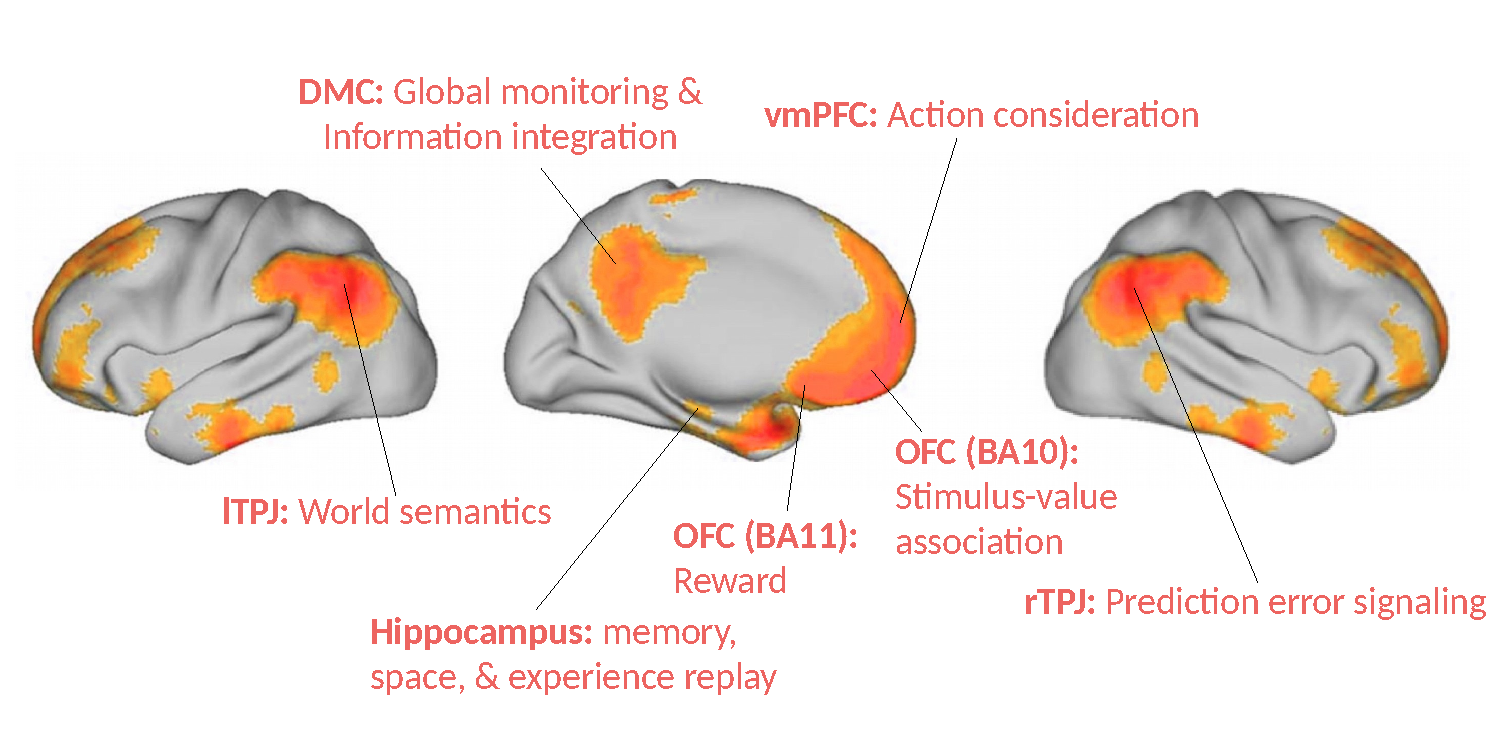
\includegraphics[width=.9\linewidth]{neurobiological_overview_DMN.pdf}
  \caption{\textbf{Default mode network: key functions.}
  Neurobiological overview of the DMN with its major constituent nodes and
  the associated functional roles relevant in our functional interpretation.}
  \label{fig:neurobiological_overview_DMN}
\end{figure}
%
\subsection{The posteromedial cortex: global monitoring and information integration}
The midline structures of the human DMN,
including the posteromedial cortex (PMC) and
the medial prefrontal cortex (mPFC),
are probably responsible for the highest turn-over
of energy consumption \citep{raichle2001pnas, raichle_baseline}.
These metabolic characteristics go hand-in-hand with
neuroimaging analyses that suggested the PMC and mPFC to
potentially represent the functional backbone of the DMN
\citep{andrews2010, hagmann2008mapping}.


Normal and disturbed metabolic fluctuations in the
human PMC have been closely related to
changes of conscious awareness \citep{cavanna2006precuneus}.
Indeed,
the PMC matures relatively late (i.e., myelination) during postnatal development in monkeys
\citep{goldman1987development}, which is generally considered to
be a sign of evolutionary sophistication.
%
This DMN region has long been speculated to
reflect constant computation of
environmental statistics and its internal representation
as an inner ``mind's eye'' \citep{cavanna2006precuneus, leech_pcc2014}.
For instance, B\'alint's syndrome is a neurological disorder of conscious
awareness that results from medial damage in the parietal cortex
\citep{balint1909seelenlahmung}.
Neurological patients are plagued by an
inability to combine various individual features of the visual
environment into an integrated whole (i.e., simultanagnosia)
as well as an inability to direct action towards
currently unattended environmental objects
(i.e., optic ataxia).
This can be viewed as a high-level impairment in gathering
information about alternative objects (i.e., exploration) as well as
leveraging these environmental opportunities (i.e., exploitation).
Congruently,
the human PMC was coupled in two functional connectivity analyses
\citep{bzdok2015subspecialization}
with the amygdala, involved in significance evaluation, and
the nucleus accumbens (NAc), involved in reward evaluation.
Specifically, among all parts of the PMC,
the ventral posterior cingulate cortex was
most connected to the laterobasal
nuclei group of the amygdala
\citep{bzdok2015subspecialization}.
This amygdalar subregion has been proposed to
continuously scan environmental input
for biological relevance assessment
\citep{amygdala_bzdok}.


The putative role of the PMC in continuous abstract integration of
environmental relevance
and ensuing top-level guidance of action on the environment is supported
by many neuroscience experiments.
Electrophysiological recordings in animals implicated PMC neurons in
strategic decision making \citep{pearson2009neurons},
risk assessment \citep{mccoy2005risk},
outcome-dependent behavioral modulation \citep{hayden2009electrophysiological},
as well as approach-avoidance behavior
\citep{vann2009does}.
Neuron spiking activity in the PMC allowed distinguishing
whether a monkey would pursue an exploratory or exploitative
behavioral strategy during food foraging \citep{pearson2009neurons}.
Further, single-cell recordings in the monkey PMC
demonstrated this brain region's sensitivity to
subjective target utility \citep{mccoy2005risk} and integration
across individual decision-making instances \citep{pearson2009neurons}.
This DMN region encoded the
preference for or aversion to options with uncertain reward outcomes
and its spiking activity was more associated with
subjectively perceived relevance of a chosen object
than by its actual value,
based on an ``internal currency of value'' \citep{mccoy2005risk}.
In fact, direct stimulation of PMC neurons
promoted exploratory actions,
which would otherwise be shunned \citep{hayden2008stim}.
Graded changes in firing rates of PMC neurons
indicated changes in upcoming choice trials, while their neural patterns were
distinct from neuronal spike firings that indicated choosing either option.
Similarly in humans,
the DMN has been shown to gather and integrate information
over different parts of auditory narratives in an fMRI study
\citep{simony2016dynamic}.


Moreover, the retrosplenial portion of the PMC could support
representation of action possibilities
and evaluation of reward outcomes by integrating
information from memory recall and different perspective frames.
Regarding memory recall, retrosplenial damage has been
consistently associated with anterograde and retrograde memory impairments
of various kinds of sensory information
in animals and humans
\citep{vann2009does}.
Regarding perspective frames, the retrosplenial subregion of the PMC has been
proposed to mediate between the organism's egocentric
(i.e., focused on sensory environment) and
allocentric (i.e., focused on world knowledge) viewpoints
in animals and humans
\citep{epstein2008parahippocampal, burgess2008spatial, valiquette2007different}.



Consequently, the PMC may contribute to overall DMN function
by monitoring the subjective outcomes
of possible actions and integrating that information
with memory and perspective frames
into short- and longer-term behavioral agendas.
Estimated value, that differs across individuals, might enrich
statistical assessment of the environment
to map and predict delayed reward opportunities in the future.
In doing so, the PMC may continuously adapt the organism to changes
in both the external environment and its internal representation
to enable strategic behavior.


\subsection{The prefrontal cortex: action consideration and stimulus-value association}
Analogous to the PMC,
the dorsomedial PFC (dmPFC) of the DMN is believed to subserve
multi-sensory processes
across time, space, and content domains to
exert top-level control on behavior.
Comparing to the PMC, however,
dmPFC function may be closer to a
``mental sketchpad'' \citep{goldman1996prefrontal}, as it
potentially subserves the de-novo construction and manipulation
of meaning representations instructed by stored semantics and memories
\citep{bzdok2013segregation}.
The dmPFC may subserve inference, representation, and assessment
of one's own and other individuals' action considerations.
Generally,
neurological patients with tissue damage in the prefrontal cortex
are known to struggle with
adaptation to new stimuli and events
\citep{stuss1986frontal}.
Specifically, neural activity in the human dmPFC
reflected expectations about other peoples' actions and
outcomes of these predictions.
Neural activity in the dmPFC indeed explained the performance decline
of inferring other peoples' thoughts in aging humans \citep{moran2012social}.
Certain dmPFC neurons in macaque monkeys exhibited a preference
for processing others', rather than own, behavior
with fine-grained adjustment of contextual circumstances \citep{yoshida2010neural}.
% In fact, the spatially neighboring dorsal anterior cingulate cortex
% has also been linked to computing values and efforts of
% persisting a behavioral plan versus switching the
% environmental context in several lesion studies \citep{kolling2016value}.
%
% Such highly abstract neural computations necessarily rely on the
% construction of probabilistic internal information drawing from
% memory recall, mental scene elaboration processes,
% and stored knowledge of world regularities.
% %
% Moreover,
% in a computational neuroimaging experiment,
% dorsomedial PFC activity preferentially processed the consequences of
% action choices that were considered but not actually executed,
% whereas ventromedial PFC (vmPFC) activity
% processed especially value outcomes of actions actually performed on the environment
% \citep{nicolle2012agent}.


Comparing to the dmPFC,
the vmPFC probably subserves
subjective value evaluation and
risk estimation of relevant environmental stimuli
(see Fig. \ref{fig:neurobiological_overview_DMN} and \ref{fig:dmn}).
The ventromedial prefrontal DMN may
subserve adaptive behavior by bottom-up-driven
processing of “what matters now”,
drawing on sophisticated value representations
\citep{rolls_OFC, doherty2015structure}.
Quantitative lesion findings across 344 human individuals confirmed
a substantial impairment in value-based action choice
\citep{glascher2012lesion}.
Indeed,
this DMN region is preferentially connected with reward-related and limbic regions.
The vmPFC is well known to have direct connections
with the NAc
in axonal tracing studies in monkeys \citep{haber1995orbital}.
Congruently, the gray-matter volume of the vmPFC and NAc
correlated with indices of value-guided behavior and reward attitudes
in humans
\citep{lebreton2009automatic}.
NAc activity is thought to reflect reward prediction signals
from dopaminergic neurotransmitter pathways
\citep{schultz1998predictive}
that not only channel action towards basic survival needs but also
enable more abstract reward processings, and thus perhaps RL,
in humans \citep{doherty2015structure}.

% \begin{wrapfigure}{r}{.4\linewidth}
\begin{figure}[!htbp]
  \begin{minipage}[c]{0.63\textwidth}
    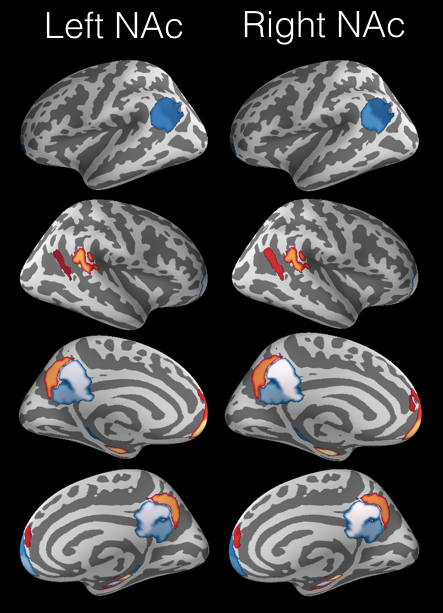
\includegraphics[width=.8\linewidth]{fig_dmn.png}
  \end{minipage}
  \hspace{-4em}
  \begin{minipage}[c]{0.45\textwidth}
    \caption{\textbf{Morphological coupling between reward system and
        default mode network.} Based on 9,932 human subjects from the UK Biobank, inter-individual differences in left NAc volume ($R^2=0.11 \pm 0.02$) and right NAc volume ($R^2=0.14 \pm 0.02$) could be predicted from volume in the DMN regions. These out-of-sample generalization performances were obtained from support vector regression applied to normalized region volumes in the DMN in a 10-fold cross-validation procedure.
      Consistent for the left and right reward system, NAc volume in a given subject is
      positively coupled with the vmPFC and HC. The colors are indicative of the (\textcolor{red}{red} = positive,
      \textcolor{blue}{blue} = negative) and relative importance (the lighter the higher) of the regression coefficients.
  Code and data for reproduction and visualization:
  \url{www.github.com/banilo/to_be_added_later}.
  }
  \label{fig:dmn}
\end{minipage}
% \end{wrapfigure}
\end{figure}

Consistently, diffusion MRI tractography in humans and monkeys
\citep{croxson2005quantitative}
quantified the NAc to
be more connected to the vmPFC than dmPFC in both species.
Two different functional connectivity analyses in humans also strongly connected
the vmPFC with the NAc, hippocampus (HC),
and PMC \citep{bzdok2015subspecialization}.
%
In line with these connectivity findings in animals and humans,
the vmPFC is often proposed to represent triggered
emotional and motivational states \citep{damasio1996somatic}.
Such real or imagined arousal states could be mapped in the vmPFC
as a bioregulatory disposition influencing cognition
and decision making.
In neuroeconomic studies of human decision making,
the vmPFC consistently reflects an individual’s subjective
value estimates
\citep{behrens2008associative}.
This may be why performance within and across participants
was related to state encoding in the vmPFC \citep{Schuck2016}.
Such a ``cognitive map'' of the action space was argued to encode
the current task state even when states are unobservable from
the sensory environment.

\subsection{The hippocampus: memory, space, and experience replay}
The DMN midline has close functional links
with the HC in the medial temporal lobe \citep{vincet2006, shannon2013morning} \textemdash
a region long known to be involved in
memory operations and spatial navigation in animals and humans.
While the HC
is traditionally believed to allow recalling past experience,
there is now increasing evidence for an important role
in constructing mental models in general
\citep{maguire2016, schacter2007remembering, gelbard2008internally, Javadi2017,
boyer2008evolutionary}.
Its recursive anatomical architecture
may be specifically designed to allow reconstructing
entire sequences of experience from memory fragments.
Indeed,
hippocampal damage is
not only associated with an impairment in re-experiencing the past (i.e., amnesia),
but also imagination dedicated to one's own future and
imagination of experiences more broadly \citep{hassabis2007patients}.

Mental scenes created by neurological patients with HC lesion exposed a lack of
spatial integrity, richness in detail, and overall coherence.
%
Single-cell recordings in the animal HC revealed
constantly active neuronal populations whose firing coincided with
specific locations in space during environmental navigation.
Indeed, when an animal is choosing between alternative
paths, the corresponding neuronal populations in the HC
spike one after another  \citep{johnson2007neural}.
Such neuronal patterns in the HC appear to directly indicate upcoming behavior,
such as in planning navigational trajectories
\citep{pfeiffer2013hippocampal} and
memory consolidation of choice relevance \citep{lavilleon2015}.
Congruently,
London taxi drivers, humans with high performance in spatial navigation,
were shown to exhibit increased gray-matter volume in the
HC \citep{maguire2000navigation}.


There is hence increasing evidence that
HC function extends beyond simple forms of
encoding and reconstruction of memory and space information.
Based on spike recordings of hippocampal neuronal populations,
complex spiking patterns can be followed across extended periods including
their modification of input-free self-generated patterns
after environmental events \citep{buzsaki2004large}.
Specific spiking sequences, which were elicited by experimental task design,
have been shown to be re-enacted spontaneously during
quiet wakefulness and sleep \citep{hartley2014space, o2010play}.
Moreover, neuronal spike sequences measured in hippocampal place cells of rats
featured re-occurrence directly after experimental trials
as well as directly before upcoming experimental trials \citep{diba2007forward}.
Similar spiking patterns in hippocampal neurons during rest and sleep
have been proposed to be critical in communicating local information
to the neocortex for long-term storage, potentially also in the regions of the DMN.
Moreover, in mice, invasively triggering spatial experience recall
in the HC during sleep
has been demonstrated to subsequently alter action choice during wakefulness
\citep{lavilleon2015}.
These HC-subserved mechanisms
conceivably contribute to advanced cognitive processes that require
re-experiencing or newly constructed mental scenarios,
such as in recalling autobiographical memory episodes
\citep{hassabis2007patients}.
Thus, the HC would orchestrate re-experience of environmental aspects for
consolidations based on re-enactment and for integration into
rich mental scene construction \citep{deuker2016event, bird2010establishing}.
As such, the HC may impact
ongoing perception of and action on the environment
\citep{maguire2016, lavilleon2015}.
% (TODO: relate to self-play in deepmind Go).
% (TODO: Kai had an interesting idea: the deja-vu effect
% could be when you already accidentally perturbed past
% such that it really occures in reality later.)


\subsection{The right and left TPJ: prediction error signaling and world semantics}
The DMN emerges with its midline structures early in human development
\citep{doria2010}, while
the right and left TPJs may become fully integrated into this major brain
network only after birth.
The TPJs are known to exhibit hemispheric differences
based on microanatomical properties and gyrification patterns
\citep{seghier2013angular}.
Globally, neuroscientific investigations on hemispheric functional specialization
have highlighted the right versus left cerebral hemisphere as dominant for
attentional versus semantic functions
\citep{seghier2013angular, bzdok2013tpj, bzdok2016left,
stephan2007mechanisms}.



The TPJ in the right-hemispheric DMN (RTPJ)
has been shown to be closely related to
multi-sensory prediction and prediction error signaling.
It is central for action initiation during goal-directed psychological tasks and for
sensorimotor behavior by integrating multi-sensory attention
\citep{corbetta2002control}.
Involvement of this DMN region was repeatedly reported in
multi-step action execution \citep{hartmann2005takes},
visuo-proprioceptive conflict \citep{Balslev2005}, and
detection of environmental changes across
visual, auditory, or tactile stimulation
\citep{downar2000multimodal}.
Direct electrical stimulation of the human
RTPJ during neurosurgery was associated with altered perception
and stimulus awareness \citep{blanke2002neuropsychology}.
%
It was argued that the RTPJ encodes actions and ensuing outcomes,
without necessarily relating those to value estimation
\citep{liljeholm2013neural, hamilton2008action,
jakobs2009effects}.
Additionally, neural activity in the RTPJ has been proposed to reflect
stimulus-driven attentional reallocation to
self-relevant and unexpected sources of information
as a ‘‘circuit breaker’’ that recalibrates functional control of brain networks
\citep{bzdok2013tpj, corbettashul2008}.
% (Bzdok et al., 2013; Corbetta et al., 2008).
Indeed, neurological patients with RTPJ damage have particular difficulties
with multi-step actions \citep{hartmann2005takes}.
In the face of large discrepancies between actual and previously predicted
environmental events the RTPJ acts as a potential switch between
externally-oriented mind sets focussed on the
sensory environment and internally-oriented mind sets focussed
on mental scene construction.
For instance, temporally induced RTPJ damage in humans diminished the
impact of predicted intentions of other individuals
\citep{young2010disruption},
a capacity believed to be enabled by the DMN.
The RTPJ might hence be an important relay that shifts away
from the ‘‘internally directed’’ baseline processes
to, instead, deal with unexpected environmental stimuli and events.
% (TODO: slow endogeneous changes in state transitions by the policy and value matrices)



The TPJ in the left-hemispheric DMN (LTPJ),
in turn, has a close relationship to Wernicke's area
involved in semantic processes, such as in spoken and written language.
Neurological patients with damage in Wernicke's area
have a major impairment of language comprehension
when listening to others or reading a book.
Patient speech
preserves natural rhythm and normal syntax, yet the
voiced sentences lack meaning (i.e., aphasia).
Abstracting from speech interpretations in linguistics
and neuropsychology,
the LTPJ mediates access to and integration of world knowledge,
such as required during action considerations
\citep{binder2011neurobiology, seghier2013angular}.
Consistent with this view,
LTPJ damage in humans also entails problems in recognizing
others' pantomimed action towards objects
without obvious relation to processing explicit language content
\citep{varney1987locus}.
% (Varney and Damasio 1987; Rothi et al. 1991; Buxbaum et al. 2005).
%
Inner speech also hinges on knowledge recall
about the physical and social world.
Indeed,
the internal production of
verbalized thought (``language of the mind'') was closely related to the LTPJ
in a pattern analysis of brain volume
\citep{geva2011neural}.
Further,
episodic memory recall and mental imagery strongly draw on
re-assembling world knowledge.
Isolated building blocks of world structure get rebuilt
in internally constructed mental scenarios that
guide present action choice,
weigh hypothetical possibilities, and forecast future events.
%
The LTPJ may hence facilitate the automated environmental predictions
by incorporating experience-derived building blocks of world regularities
into ongoing action, planning, and problem solving.
% world -> policy matrix driven computation
% self -> value matrix driven computation



\section{Reinforcement learning control: a process model for DMN function}
We now argue the outlined neurobiological properties
of the DMN regions
to be sufficient for implementing all components
of a full-fledged reinforcement-learning (RL) system.
Recalling past experience, considering candidate actions,
random sampling of possible experiences, as well as
estimation of instantaneous and expected delayed reward outcomes
are key components of intelligent RL agents
that are plausible to functionally intersect in the DMN.

RL is an area of machine learning concerned with learning optimal behavioral through interactions
with an \textit{environment}, the goal being to maximize some notion of \textit{cumulative reward}.
The optimal behavior typically
takes the future into account, as some rewards could be \textit{delayed}.
Through repeated interactions with the environment,
the agent learns to reach goals and optimize reward signals
in an iterative trial-and-error fashion (Fig. \ref{fig:rl}).
At a given moment, each taken \textit{action} $a$ triggers a change
in the \textit{state} of the environment
$s \rightarrow s'$, accompanied by environmental feedback signals as \textit{reward}
$r = r(s, a,s')$ collected by the agent.
If the collected reward outcome yields a negative value it can be
more naturally interpreted as \textit{punishment}.
In this view, the environment is partially controlled by
the action of the agent and the reward can be thought
of as satisfaction \textemdash or aversion \textemdash accompanying the execution of
a particular action.
% Action may be delayed to achieve substantial increases in expected reward
% that is expected to grow with time.

The environment is generally taken as \textit{stochastic},
that is, changing in random ways. In addition, the environment is only
\textit{partially observable} in the sense that only limited aspects of the environment's
state are accessible to the agent's sensory perception.
\citep{starkweather2017dopamine}.
We assume that volatility of the environment
is realistic in a computational model which sets out
to explain DMN functions of the human brain.
% XXX: the following passage is already in the introduction
% Indeed, it is known that the more the external world is predictable,
% the more mental activity becomes detached from the actual sensory inputs
% \citep{antrobus1966studies, pope1978regulation},
% the more stimulus-independent thoughts occur, and
% the higher the neural activity in the DMN.
% Conversely, the more the currently executed task is unknown and unpracticed,
% the lower the DMN activity
% \citep{filler1973daydreaming, teasdale1995stimulus}.
% %
% These ``offline'' processes may however contribute to
% optimizing control of the organism.
% Such a framework of DMN funtion based on reinforcement learning
% can naturally embed human behavior
% in the tension between exploitative action with immediate gains and
% explorative action with longer-term reward schedules
% \citep{dayan2008decision}.
We argue that a functional account of the DMN based on RL
can naturally embed human behavior
in the tension between exploitative action with immediate gains and
explorative action with longer-term reward outcomes
\citep{dayan2008decision}.
In short, DMN implication in a diversity of
particularly advanced cognitive processes
can be parsimoniously explained as probabilistic mental
scene of experience simulations coupled with prediction error minimization
to calibrate action trajectories for
reward outcome maximization at different time scales.
Such a purposeful optimization objective
may be solved by a stochastic approximation
based on a brain implementation of MCMC sampling
\citep{tenenbaum2011grow}.

\begin{figure}[!h]
  \centering
  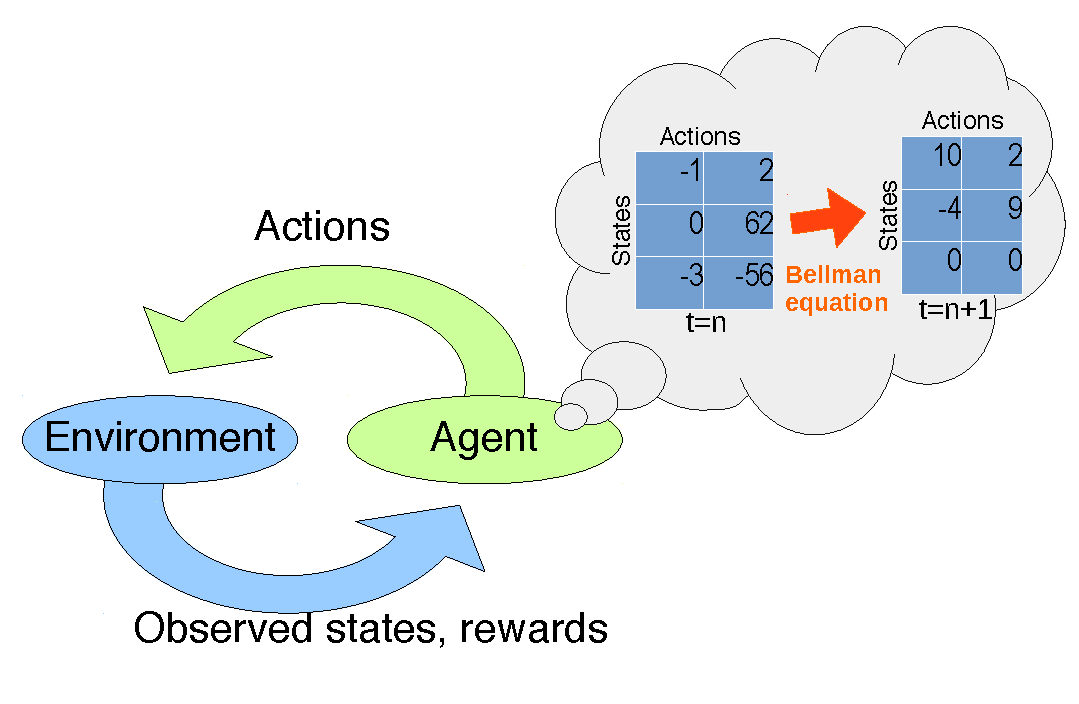
\includegraphics[width=1.\linewidth]{rl2.pdf}
  \caption{\textbf{Reinforcement learning in a nutshell.} Given the current state of the environment,
    the agent takes an action by following the policy matrix as updated by the Bellman equation. The agent receives a consequential reward and observes the next state. The process goes on until interrupted or a goal state is reached.}
  \label{fig:rl}
\end{figure}

\subsection{Markov decision processes}
Reinforcement learning (RL) has had great success in many real-world problems, including robotics \citep{ng2004,abbeel2004},
super-human performance in complex video games \citep{mnih2015},
and strategic board games like the breakthrough results upon recently on the game of Go \citep{silver2016mastering}, considered to be a golden benchmark problem in artificial intelligence.
We emphasize that the brain in general, and the DMN in particular,
is a physical system governed by the laws of
physics and can be formally described
by Markov processes at a sufficiently coarse scale.
It has indeed been previously proposed \citep{tegmark2016improved} that
any system obeying the laws of classical physics can be accurately modeled as a Markov process as long as the time
step is sufficiently short.

In artificial intelligence and machine learning, a popular computational model for
multi-step decision processes in such an environment are
\textit{Markov decision processes} (MDPs) \citep{sutton1998reinforcement}.
% For the remainder of this paper, for the sake of simplicity
% we use the abbreviation ``MDP'' to refer to the special case
% of \textit{Partially Observable Markov Decision Processes}.
An MDP operationalizes a sequential decision process
in which it is assumed that environment dynamics are determined by a Markov process,
but the agent cannot directly observe the underlying state.
Instead, the agent tries to optimize a \textit{subjective} reward
signal (i.e., is likely to be different for another agent in the same state),
by maintaining probability distributions over actions according to their expected utility.
% This is performed alongside each transition in the state space of the environment
%  and maintains a probability distribution over the set of possible
% states.
% % , based on a set of observations and observation probabilities.
This is a minimal set of assumptions that can be made about an environment faced by an agent engaged in active learning.

\begin{definition*}
Mathematically, an MDP is simply a quintuplet $(\mathcal S, \mathcal A, r, p)$ where
\begin{itemize}
\item $\mathcal S$ is the set of states, such as $\mathcal S = \{\text{happy}, \text{sad}\}$.
\item $\mathcal A$ is the set of actions, such as $\mathcal A = \{\text{read}, \text{run},
  \text{laugh}, \text{sympathize}, \text{empathize}\}.$
\item $r : \mathcal S \times \mathcal A \times \mathcal S \rightarrow \mathbb R$ is the \textit{reward function},
   so that $r(s, a, s')$ is the instant reward for taking action $a$ in state $s$ followed by a state-transition $s \rightarrow s'$.
% \item $\mu: \mathcal S \rightarrow [0, 1]$ is the prior probability on the states so that
%   $\mu(s)$ is the probability that the environment starts off in state $s$.
\item $p : \mathcal S \times \mathcal A \times \mathcal S \rightarrow [0, 1],\; (s,a,s') \mapsto p(s'|s,a)$,
  the probability of moving to state $s'$ if action $a$ is taken from state $s$. In addition, one requires that such
  transitions be Markovian. Consequently, the future states are independent of past states and only depend on the present state and action taken.
\end{itemize}
\end{definition*}

% , defining $s(t)$, the state at time $t$, as the position in state space.
The process has $memory$ if the next state depends not only on the current state
but also on a finite number of past states.
Rational probabilistic planning can thus be reformulated
as a standard memoryless Markov process by simply expanding the
definition of the state $s$ to include experience episodes of the past.
This adds the capacity for memory, since then, the next state depends not only on the current state but also on a finite number of past states. This is precisely what Partially Observable MDPs (POMDPs) do ~\citep{starkweather2017dopamine,o2006making}.
Nevertheless, this mathematical procedure in POMDPs only accounts for implicit $memory$. Since the current paper is aiming at both plausibility at the behavioral and neural level, we will address later in the paper how our model captures the neurophysiological constraints of the DMN and can also account for the explicit part of $memory$ from a human agent perspective.

\paragraph*{Why MDPs ?} One may wonder whether MDP models are applicable to something as complex as human behavior. For instance, financial trading is largely a manifestation of strategic decision-making of interacting human agents. According to how the market responds, the agent incurs definite gain or loss as environmental feedback of the executed financial actions. Recent research on automatizing market exchanges by algorithmic trading has successfully used MDPs as a framework for modeling these sophisticated behavioral process  ~\citep{brazdil2017,yang15,yang14,yang12,dempster2006,hult2010}. ~\citep{abergel2017} is an excellent reference with the mathematical details on how MDPs can be readily exploited in the financial world.
%
MDPs have also been effective as a behavioral model in robotics \citep{ng2004,abbeel2004} and in challenging multistep strategy games ~\citep{mnih2015,silver2016mastering,pritzel2017neural}.
%
As such, we aim to expand MDPs as a useful model from "online" decision-making to the realms of "offline" mental operations most associated with the DMN.


% Indeed a critique could argue that Markov chains are state-machines without memory. These may describe insects, or other behaviorally primitive beings like ATM machines, insects, etc., but won't be sufficient to describe human beings, as for example, human behavior is heavily influenced not only by the current state but by past states as well (memory).

% \paragraph*{Answer:}
% \begin{itemize}
%   \item First, let us emphasize that the brain in general, and the DMN in particular,
% is a physical system governed by the laws of
% physics and can be formally described
% by Markov processes at a sufficiently coarse scale.
% It has indeed been previously proposed \citep{tegmark2016improved} that
% any system obeying the laws of classical physics can be accurately modeled as a Markov process as long as the time
% step is sufficiently short.



% \end{itemize}


\paragraph*{Towards Model-free reinforcement learning for the DMN.}
Model-free RL can be plausibly realized in the human brain \citep{doherty2015structure}. Indeed,
it has been proposed \citep{gershman2015computational} that a core property of human intelligence  underlie improvement
of expected utility outcomes as a strategy for action choice in uncertain
environments, a situation perfectly captured by the formalism of MDPs.
It has also long been proposed \citep{dayan2008decision} that there
is a rather direct mapping of model-free RL learning algorithms
onto aspects of the brain.
The neurotransmitter dopamine could serve
as a ``teaching signal'' to better estimate value associations
and action policies by controlling
synaptic plasticity in the reward-processing circuitry, including the NAc.
In contrast, \textit{model-based RL} would start off with some mechanistic assumptions about the dynamics of the world.
These can be assumptions about the physical laws governing the agent's environment or constraints on the state space, transition probabilities between states,
reward contingencies, etc.
% For instance, if a rat in a maze knows
% that standing still will produce no change in the environment, and in particular will not eventually lead to finding the food.
An agent might represent such knowledge about the world as follows:
\begin{itemize}
\item $r(s, \text{``stand still''}) = 0$ if $s$ does not correspond to a location
offering relevant resources.
\item $p(s'|s,\text{``stand still''}) = 1$ if $s'=s$ and $0$ otherwise.
\item etc.
\end{itemize}
% Model-based assumes knowledge of the environment in terms of the transition probabilities between states, the reward contingencies for state-action pairs, or any form of representation of the environment.
Such knowledge can of course be partly learned from the environment: the agent learns a model for the world alongside learning to make optimal decisions using this model. These methods learn what the effect is going to be of taking an particular action in a particular state. The result is an estimate of the underlying MDP which can then be either solved exactly or approximately, depending on the setting and what is feasible. The main problem then is to "connect the dots", by using dynamic programming --for example.


In contrast, model-free methods require no knowledge of the environment (transition probabilities, identities of sensory input, etc.) or representation thereof, and the agent learns which state-action pairs lead to reward through sampling the world in trial-and-error manner, and predicting long-run reward aggregates, using prediction error as an incentive. In so doing, such methods ultimately learn both a policy and  implicit representations of the world / environment. This is what algorithms TD learning~\citep{sutton1998reinforcement}. In terms of number of states, model-based RL scales better than model-free RL; in terms of the time horizon, model-free RL scales better~\citep{strehl2006}. Drawing from a vast literature, we will show that the DMN contains sufficient neurobiological hardware to implement model-free RL, at least in principle.

\subsubsection{Accumulated rewards and policies}
The behavior of the agent is governed by a \textit{policy}, which maps states of the world
to probability distributions over actions.
Starting at time $t=0$,
following a policy $\pi$ generates a trajectory of action choices as follows:
\begin{eqnarray*}
  \begin{split}
    \textbf{choose action: }a_0 &\sim \pi(a|s_0)\\
    \textbf{ observe transition: }s_1 &\sim p(s|s_0,a_0)\textbf{ and collect reward }R_0 = r(s_0, a_0, s_1)\\
    \textbf{choose action: }a_1 &\sim \pi(a|s_1)\\
    \textbf{ observe transition: }s_2 &\sim p(s|s_1,a_1), \textbf{ and collect reward }R_1 = r(s_1, a_1,s_2)\\
    \vdots\\
    \textbf{choose action: }a_{t} &\sim \pi(a|s_{t})\\
    \textbf{ observe transition: }s_{t+1} &\sim p(s|s_{t},a_{t}), \textbf{ and collect reward }R_{t} = r(s_{t}, a_{t},s_{t+1})\\
    \vdots
  \end{split}
\end{eqnarray*}
We assume time-invariance
in that we expect the dynamics of the process
to be equivalent over sufficiently long time windows of equal length (i.e., stationarity).
Since an action executed in the present moment might have repercussions in the far future, it turns out that the
quantity to optimize is not the instantaneous rewards $r(s, a)$, but a
\textit{cumulative reward} estimate which takes into account expected reward
from action choices in the future.
A common approach to
modeling this accumulation is the time-discounted cumulative reward% function
\begin{equation}
  \label{eq:cumr}
  G^\pi = \sum_{t=0}^{\infty}\gamma^{t}R_t = R_0 + \gamma R_1 + \gamma^2 R_2 + \ldots + \gamma^tR_t + \ldots
\end{equation}
This random variable\footnote{Random as it depends both on the environment's dynamic and the
  policy $\pi$ being played (which can be stochastic).}  measures the cumulative reward of
following an action policy $\pi$.
%
Note that value buffering may be realized in the vmPFC.
This DMN region has direct connections to
to the NAc, known to be involved in reward evaluation.



The goal of the RL agent is then to update this action policy in order
to maximize $G^\pi$ on average (cf. below). In \eqref{eq:cumr},
the definition of cumulative reward $G^\pi$,
the constant $\gamma$ $(0 \le \gamma < 1$) is the \textit{reward discount factor},
viewed to be characteristic for a certain agent.
On the one hand,
setting $\gamma = 0$ yields perfectly hedonistic behavior.
An agent with such a shortsighted time horizon is exclusively
concerned with immediate rewards.
This is however not compatible with coordinated planning of long-term goal that is
potentially subserved by neural activity in the DMN.
% \footnote{In which case we can take $T \rightarrow +\infty$, provided the reward function $r$ is bounded.}.
% The reward discount factor
On the other hand,
setting $0 < \gamma < 1$ allows a learning process to arise.
A positive $\gamma$ can be seen as calibrating risk-seeking trait of the intelligent agent,
that is, the behavioral predispositions related to trading longer delays
for higher reward outcomes.
Such an agent puts relatively more emphasis on rewards expected in
a longer-term future.
More specifically,
rewards that are not expected to come within
% \footnote{\textbf{N.B.:} $\frac{1}{1-\gamma} = 1 + \gamma + \gamma^2 + \gamma^3 + \ldots$}
$\tau := 1/(1 - \gamma)$
time steps from the present point are disregarded. This reduces the variance of expected rewards accumulated across
considered action cascades by limiting the depth of the search tree.
Given that there is more uncertainty in the farsighted future,
it is important to appreciate that a stochastic policy estimation
is more advantageous in many RL settings.
% For instance, a deterministic strategy in playing rock-paper-scissors can
% be easily exploited and a uniformly random choice is optimal.

\subsection{The components of reinforcement learning in the DMN}
Given only the limited information available from an MDP, at a state $s$ the average
utility of choosing an action $a$ under a policy $\pi$ can be captured by the single number
% We can now formulate the purpose of the DMN
% as finding a policy $\pi$ for the human agent that maximizes the
% expected cumulative value of an state-action pair $(a,s)$, also known as the \textit{Q-value}, namely
\begin{equation}
  \label{eq:qval}
  Q^{\pi}(s,a) = \mathbb E [G^\pi|s_0=s,a_0=a],
\end{equation}
called the $Q$-value for the state-action pair $(s,a)$.
In other words, $Q^{\pi}(s,a)$ corresponds to the expected reward
over all considered action trajectories, in which
the agent sets out in the environment in state
$s$, chooses action $a$, and then follows the policy $\pi$ to select future actions.
%% Given that each $\pi$ correspondence to an exhaustive description of
%% behavioral patterns, $Q^{\pi}(s_t,a_t)$ corresponds to the epistemic value of
%% the set of actions given states in finite time.
For the brain,
$Q^{\pi}(s, a)$ defined in \eqref{eq:qval} provides the subjective
utility of executing a specific action.
It thus answers the question
``What is the expected utility of taking action $a$ in this situation ?''.
$Q^{\pi}(s,a)$ offers a formalization of optimal behavior that
may well capture processing aspects of the DMN in human agents.

% One can also define the state-value function

% \begin{eqnarray}
%   \V^\pi(s) := \mathbb E_{a \sim \pi}Q^\pi(s,a) = \mathbb E [G^\pi|s_0=s],
% \end{eqnarray}
% which measures the value of each state $s \in \mathcal S$ under the policy $\pi$. This serves
% as a baseline value for any action. Finally, the advantage function is defined by
% \begin{equation}
% A^\pi(s,a) :=  Q^\pi(s,a) - V^\pi(s).
% \end{equation}

% The goal of the DMN is then
% to find then to produce a policy $\pi$ which maximizes the expected cumulative reward $Q^\pi(s_0,\pi(a_0))$
% given an initial state $s_0$.

% \subsection{Efficient computation of optimal behavior}
% By construction, maximizing the expectation in  \eqref{eq:qval} is computationally intractable in general.
% This is due to the enormous number of possible action
% trajectories that the agent often needs to
% consider simultaneously.
% % \begin{mdframed}
% %   \textbf{N.B.:}
% %   If the Bellman-based computational ideas have a corresponding
% %   neurobiological implementation, this provides a framework of how
% %   optimal behavior could be computable in the human brain.
% % \end{mdframed}
% One popular solution is called \text{Q-learning}. It remedies
% the issue by only considering the sub-family of
% \textit{deterministic policies}, which map each state to the single best action to
% take at the current state. Such policies define deterministic functions from states to actions.

% \subsubsection{The Bellman equation:  characterizing optimal behavior}
% Q-learning (Watkins \& Dayan, 1992) generates a
% \textit{greedy policy}
\subsubsection{Optimal behavior and the Bellman equation}

Optimal behavior of the agent corresponds to
a strategy $\pi^*$ for choosing actions such that, for every state, the chosen action guarantees the best possible reward on average. Formally,
% \textbf{XXX please add 1-2 sentences why this is interesting in the current
% context. This statement appears a little alone as it stands.}
\begin{equation}
  \pi^*(s) := \argmax_{a \in \mathcal A}{Q}^*(s, a),\text{ where }Q^*(s, a) := \max_{\pi}Q^\pi(s,a).
  \label{eq:qlearning}
\end{equation}
The learning goal is to approach the
policy $\pi^*$ as close as possible, that is to \text{solve} the MDP.
Note that \eqref{eq:qlearning} presents merely a definition and
does not lend itself as a candidate schema
for solving MDPs with even moderately-sized action and state spaces
(i.e., intractability).
% where $\tilde{Q}(s, a)$ is the current estimate of the state-action value
% table.
Fortunately, the \textit{Bellman equation} \citep{sutton1998reinforcement} provides a fixed-point relation which defines $Q^*$ implicitly via a sampling procedure, without querying the entire space of policies, with the form
\begin{equation}
  Q^* = \text{Bel}(Q^*),
  \label{eq:bellman}
\end{equation}
where the so-called Bellman transform $\text{Bel}(Q)$
of an arbitrary $Q$-value function $Q: \mathcal S \times \mathcal A \rightarrow \mathbb R$  is another $Q$-value function defined by
\begin{equation}
  \begin{split}
   \text{Bel}(Q)(s,a) &:=
   \mathbb E_{s' \sim p(s'|s,a)} [r(s,a) + \gamma \max_{a' \in \mathcal A}Q(s', a')]\\
   &= r(s,a) + \gamma\mathbb E_{s' \sim p(s'|s,a)} [\max_{a' \in \mathcal A}Q(s', a')]\\
   &= \text{instantaneous reward} + \text{expected reward for acting greedily thereafter}
%    \; \forall (s,a) \in \mathcal S \times \mathcal A
    % \\&=
    % \mathbb E_{s' \sim p(s'|s,a)} [r(s,a) + \gamma Q^*(s', \pi^*(s'))].
    \end{split}
  \end{equation}

The Bellman equation \eqref{eq:bellman} is a temporal consistency equation which provides
a dynamic decomposition of optimal behavior by dividing the $Q$-value function into the immediate
reward and the discounted rewards of the upcoming states.
The optimal Q-value operator $Q^*$ is a fixed point for this equation.
As a consequence of this decomposition, the complicated dynamic programming
problem \eqref{eq:qlearning}
is broken down into simpler sub-problems at different time points.
Indeed,
exploitation of hierarchical structure in action considerations
has previously been related to the medial prefrontal part of the DMN
\citep{koechlin1999role, braver2002role}.
Using the Bellman equation, each state can be associated with a certain value
to guide action towards a preferred state, thus improving on the
current action policy of the agent.
% It is a fixed-point equation for the deterministic policy $\pi$.
Note that in \eqref{eq:bellman} the random sampling
is performed only over quantities which
depend on the environment.
This aspect of the learning process
can unroll off-policy by observing state transitions
triggered by another (possibly stochastic) behavioral policy.

\begin{mdframed}
% neuroscience of Bellman equation
  \vspace{2em}
  \textbf{Box 1: Neural correlates of the Bellman equation in the DMN}
% \hspace{-1.5em}
Relating decomposition of consecutive action choices by the Bellman equation
to neuroscience,
specific neural activity in the dorsal prefrontal cortex (BA9)
was linked to processing ``goal-tree sequences''
in human neuroimaging experiments
\citep{koechlin1999role, koechlin2000dissociating}.
Sub-goal exploration may require multi-task switching
between cognitive processes
as later parts of a solution
frequently depend on respective earlier steps in a given solution path, which
necessitates storage of expected intermediate outcomes.
As such,
``cognitive branching'' operations for nested processing of behavioral strategies
are likely to
entail secondary reallocation of attention and working-memory resources.
Further neuroimaging experiments \citep{braver2002role} corroborated
the prefrontal DMN to subserve
``processes related to the management and monitoring of sub-goals while maintaining information in working memory''.
%
Moreover,
neurological patients with lesions in this DMN region were reported
to be impaired in aspects of realizing ``multiple sub-goal scheduling''
\citep{burgess2000cognitive}.
Hence,
the various advanced human mental abilities subserved by the DMN, such as
planning and abstract reasoning, can be viewed to involve some form of
action-decision branching to enable higher-order executive control.
\end{mdframed}


% \subsection{Learning in the DMN}
\subsubsection{Value approximation and the policy matrix}
\label{sec:policymat}
As already mentioned in the previous section, Q-learning~\citep{watkins92} optimizes over the class of
deterministic policies of the form \eqref{eq:qlearning}. State spaces may be extremely large,
and tracking all possible states and actions may require prohibitively excessive
computation and memory resources.
The need of maintaining an explicit table of
states can be eliminated by instead using of an approximate $Q$-value function $\tilde{Q}(s,a|\theta)$
by keeping track of an approximating parameter $\theta$ of much lower dimension than the number of states.
At a given time step, the world is in a state $s \in \mathcal S$, and the agent takes an
action which it expects to be the most valuable on average, namely

\begin{equation}
  \pi^{\text{hard-max}}(s) = \argmax_{a \in \mathcal A}\tilde{Q}(s, a|\theta),
  \label{eq:policy}
\end{equation}
This defines a mapping from states directly to actions.
% $a \mapsto \tilde{Q}(a,s|\theta)$ of the $Q$-value function ``frozen'' at state $s$.
For instance, a simple linear model with a kernel $\phi$ would be of the
form $\tilde{Q}(s, a|\theta) = \phi(s,a)^T\theta$, where
$\phi(s,a)$ would represent a high-level representation of the state-action pairs
$(s,a)$, as was previously proposed \citep{songNIPS2016},
or artificial neural-network models as demonstrated in recent
seminal investigations
\citep{mnih2015,silver2016mastering} for playing complex games (atari, Go, etc.) at super-human levels.
%  and Parr et al. 2003 (JMLR)].
In the DMN, the dmPFC would implement such a hard-max lookup
over the action space.
The model
parameters $\theta$ would correspond to synaptic weights and connection strengths within and between
brain regions. It is a time-varying neuronal program which dictates how to move from world states $s$ to actions $a$ via the hard-max policy \eqref{eq:policy}.
The approximating $Q$-value function $\tilde{Q}(s, a|\theta)$ would tell the DMN the (expected) usefulness of taking an action $a$ in state $s$.
The DMN, and in particular its dmPFC node, could then contribute to the choice, at a given state $s$, of an action $a$ which maximizes these approximate
$Q$-values.
This mapping from states to actions that is conventionally called
\textit{policy matrix} \citep{mnih2015,silver2016mastering}.
Learning consists in starting from a given table and
updating it during action choices,
which take the agent to different table entries.


% An additional layer of learning concerns the addition of new entries in the table (i.e., state and action). The framing of the policy matrix is not described here but could be supported by synaptic epigenesis \citep{gisiger_acquisition_2005}. Indeed, the tuning of synaptic weights through learning can stabilize additional patterns of activity by
% creating new attractors in the neural dynamics landscape \citep{takeuchi_synaptic_2014}. Those attractors will then constrain both
% the number of factors taken into account by decision processes and the number of behaviors at reach by the agent \citep{wang_decision_2008}.

% \subsubsection{Bounded rationality}
% $$\max_{a \in \mathcal A}\tilde{Q}(s, a|\theta)  \propto \lim_{T \rightarrow 0^+}\exp(\tilde{Q}(s,a|\theta)/T)$$

  \subsubsection{Self-training and the loss function}
  \label{sec:self}
Successful learning in brains and computer algorithms is not possible without a
defined learning goal \textemdash the \textit{loss function}.
The action $a$ chosen in state $s$ according to the policy matrix defined in
\eqref{eq:policy} yields a reward $r$ collected by the agent,
% (measured on their internal currency of worldly values ?),
after which the environment transitions to a new state $s' \in \mathcal S$.
% \textbf{XXX Please try to smoothen the previous sentence}
One such cycle yields a new \textit{experience} $e = (s,a,r,s')$.
Each cycle represents a behavior unit of the agent
and is recorded in replay memory buffer \textemdash
which we hypothesize to be subserved by the
HC \textemdash, possibly discarding the oldest entries to make space:
$\mathcal D \leftarrow \text{append}(\mathcal D, e)$.
At time step $k$, the agent seeks an update $\theta_{k} \leftarrow \theta_{k-1} + \delta \theta_{k}$ of the parameters for its approximate model of the $Q$-value function. This warrants a learning process
and definition of a loss function.
% \subsubsection{Stochastic gradient in the DMN via experience replay}
The Bellman equation \eqref{eq:bellman} provides a way to obtain such a loss function \eqref{eq:oracle} as we outline in the following.
% A practically successful RL approach
% needs ways to efficiently approximate the state-action value function
% to allow for scaling to large state and action spaces.
Experience replay consists in sampling
% (uniform or importance-weighted
% \footnote{e.g weighted by TD error of the state transition $s \overset{a}{\rightarrow} s'$.})
batches of experiences $e$
$(s, a, r, s') \sim \mathcal D$ from the replay memory $\mathcal D$.
The agent then tries to approximate
the would-be $Q$-value for the state-action pair $(s,a)$ as predicted by the Bellman equation \eqref{eq:bellman}, namely
\begin{equation}
  y_k := y_k(s,a,s') =  r + \gamma \max_{a'} \tilde{Q}(s', a'|\theta_{k-1}),
\end{equation}
with the prediction of a parametrized regression model $(s,a)
\mapsto \tilde{Q}(s, a|\theta_{k-1})$.
From a neurobiological perspective,
experience replay can be manifested as the re-occurrence of
neuron spiking sequences that have also occurred during specific prior actions
and environmental states.
%, but the replay has a much faster time scale.
The HC is a strong candidate to contribute to such a mechanism
because neuroscience experiments have repeatedly indicated
in rats, mice, cats, rabbits, songbirds, and
monkeys \citep{buhry2011,nokia2010,dave2000,skaggs2007}.

At the current step $k$, computing an optimal parameter update then corresponds to
finding the model parameters $\theta_{k}$ which minimize the following mean-squared loss function
\begin{equation}
  \mathcal L(\theta^Q_{k})
  % = \mathbb E_{(s, a, r, s') \sim \mathcal D}[(\tilde{Q}(s, a|\theta) - \tilde{Q}(s',a'|\theta^Q_{k}))^2]
  = \mathbb E_{(s, a, r, s') \sim \mathcal D}\left[\frac{1}{2}(\tilde{Q}(s, a|\theta_{k}) - y_k)^2\right],
  \label{eq:oracle}
\end{equation}
where $y_k$ is defined in \eqref{eq:bellman}.
% \textbf{We still may need to explain y in the formula with one sentence.}
A recently proposed, practically successful alternative approach is, to learn this
representation using an artificial deep neural-network model, leading to the
so-called \textit{deep Q-learning}~\citep{mnih2015,silver2016mastering} family of methods which
is the current state-of-the-art in RL research.
The set of model parameters $\theta$ that instantiate the non-linear interactions
between layers of the artificial neural network
may find a neurobiological correspondence in the adaptive strengths of axonal
connections between neurons from the different levels
of the neural processing hierarchy
\citep{mesulam1998sensation, taylor2015global}.

\paragraph*{Self-training may introduce bias. How to alleviate it ?}
As pointed out by one of the reviewers, self-training may introduce bias due to information shortage caused by the absence of external stimulus (task).
 way to solve this issue is to use importance sampling as was done in ~\citep{schaul2015} and ~\citep{hessel2017}, to replay more often state-transitions from which there is more to learn. New transitions are inserted into the replay buffer with maximum priority, providing a bias towards recent transitions. Such an insertion bias would help counter-balance the bias introduced by the information shortage caused by the absence of external stimulus (task). Also, ~\citep{hessel2017} noticed that such prioritized replay reduces the data-complexity and the agent can start learning much sooner than conventionally.


\subsubsection{Optimal control via stochastic gradient descent in the DMN}
Efficient learning of the entire set of model parameters can effectively be achieved
via stochastic \textit{gradient descent}, a universal algorithm for finding
local minima based on the first derivative of the optimization objective.
Stochastic here means that the true gradient is estimated from batches of training samples,
which, in our case, corresponds to blocks of experience from the replay memory:

% online stochastic gradient descent is used to minimize the variational objective
% \eqref{eq:oracle}.

% \paragraph{Parameter update.}
\begin{equation}
  \delta= -\alpha_k \nabla_{\theta_{k}}\mathcal L(\theta_{k})
  = -\alpha_k\mathbb E_{(s, a, r, s') \sim \mathcal D}[\underbrace{(\tilde{Q}(s, a|\theta_{k}) - y_k)}_{\text{prediction error}}
    \underbrace{\nabla_{\theta_{k}}\tilde{Q}(s, a|\theta_{k})}_{\text{aversion}}],
  \label{eq:oracle}
\end{equation}
where the positive constants $\alpha_1, \alpha_2,\ldots$ are learning rates.
Thus, the next action is taken to drive reward prediction errors
to percolate from lower to higher processing layers to modulate the
choice of future actions. It is a standard result that under special conditions on the learning rates $\alpha_k$ --namely that the learning rates are neither too large nor too small, or more precisely that the sum $\sum_{k=0}^\infty\alpha_k$ diverges while $\sum_{k=0}^\infty\alpha_k^2$--
the thus generated approximating sequence of $Q$-value functions
% \footnote{The proof is standard and relies on the Banach Fixed-Point Theorem applied to the Bellman transform.}
$$\tilde{Q}(.,.|\theta_0) \rightarrow \tilde{Q}(.,.|\theta_1) \rightarrow \tilde{Q}(.,.|\theta_2) \rightarrow \ldots$$
are attracted and absorbed by the optimal $Q$-value function $Q^*$ defined implicitly by the Bellman equation \eqref{eq:bellman}.

% \paragraph{Link to classical reinforcement learning.}
% One should note that most classical RL algorithms, including \textit{Temporal Difference (TD)}
% learning \citep{sutton1998reinforcement}, REINFORCE \citep{williams1992}, and SARSA can be
% cast in the general variational framework \eqref{eq:oracle}. For instance, TD corresponds to
% the above framework using a linear value approximator with feature encoding
% $\phi(s,a) = \delta_{(s,a)} =  \text{ point mass at }(s,a)$ on the grid
% $\mathcal S \times \mathcal A$, and so
% $$\nabla_{\theta}\tilde{Q}(s, a|\theta) = \phi(s, a) = \delta_{(s,a)}.$$
% Hence, the gradient update due to the sample $(s,a,r,s') \in \mathcal D$ is
% $$\tilde{Q}(s, a) \leftarrow \tilde{Q}(s, a) + \alpha(y-\tilde{Q}(s, a)),$$
% the well-known TD update rule \citep{sutton1998reinforcement}.

\subsubsection{Does the hippocampus subserve MCMC sampling?}
In RL, MCMC simulation is a common means to update the agent's belief state.
% \citep{silver2010monte}.
MCMC simulation provides a simple method for evaluating the value of a state.
They provide an effective mechanism both for tree search (of the considered
action trajectories)
and for belief state updates, breaking the curse of dimensionality and allowing much greater scalability than an RL agent without stochastic resampling procedures.
Such methods have scaling as a function of available data (i.e., sample complexity) that
is determined only by the underlying difficulty of the MDP, rather than the size of the state space or observation space,
which can be prohibitively large.

In the human brain,
the HC could contribute to synthesizing imagined sequences of world states,
actions and rewards \citep{aronov2017, chao2017interaction, boyer2008evolutionary}.
These simulations of experience batches
would be used to update the value function, without ever looking inside the black box describing the model's dynamics \citep{lavilleon2015}.
This would be a simple control algorithm by evaluating all legal actions and selecting the action with
highest expected cumulative rewards.
In MDPs, MCMC simulation provides an effective mechanism both for tree search and for belief-based state updates, breaking the curse of dimensionality and allowing much greater scalability than has previously been possible \citep{silver2016mastering}.
% Much recent work points to MCMC or stochastic sampling-based approximations as a unifying framework for understanding how Bayesian inference may work practically across all these levels, in minds, brains, and machines. \textbf{XXX elvis: refs needed in last sentence. Plus, should be really bring up Bayesian?}

\paragraph*{On implicit and explicit memory in the current model.}
Markov Processes are memoryless but this is possible mathematically to artificially insert the previous states of such model into the current state. While this may partially account for implicit memory at the behavioral level, it does not explain the underlying implementation at the neurophysiological level nor accounts for the explicit part of memory.
First, it is possible to incorporate explicit memory capacities into the MDP.

 We address this question in the paper by clarifying what memory retrieval would mean in the current account. In fact, implicit memory-based processing is already present in our MDP account of DMN function. It occurs in 3 three different forms: a) the action policy, b) the value function $\textemdash$as both of these are a result/product of the past$\textemdash$ and c) the deep architecture with many non-linear links in the hierarchical connections as realized by biological neural networks. Indeed, we reason about the brain has deep neural networks that present an implicit form of information compression obtained from life experience. This memory traces are implicitly stored in the neural machinery and can be retrieve as a form of Knowledge by simulation of action rather than accessed as a stored explicit representation \citep{pezzulo2011grounding}. The neural processes in the hippocampus can be seen as MCMC sampling from a formal statistical level but those memory recall are also the basis for scene construction processes across time-scales such as in the semantic hypothesis \citep{schacter2007remembering}. In a complementary way, neural encoding of reward information is not limited to value but incorporates specific information about the identity of the reward outcome, the predictive stimulus, or the action necessary to obtain the reward \citep{kahnt2017decade}.

\subsection{Putting everything together}
The DMN is today known to consistently increase in neural
  activity when humans engage in cognitive processes that are detached from
  the current sensory environment. Additionally,
  this network was proposed to be situated
  at the top of the brain network hierarchy, with
  the subordinate salience and dorsal attention network in the middle and
  the unimodal sensory cortices at the bottom
  \citep{carhart2010default, margulies2016situating}.
  Its putative involvement in thinking about the past,
  hypothetical experiences, and the future
  appears to tie in with the implicit computation of
  action and state cascades as a function of what happened in the past.
  A policy matrix encapsulates the repertoire of possible actions
    on the world given a current state.
    The policy matrix encodes the probabilites of
    choosing actions to be executed in a certain situation.
The DMN may subserve
  constant exploration of possible action trajectories and
  nested estimaton of their
  cumulative reward outcomes. Implicit computation of future choices
  provides an explanation for the
  evolutionary emergence and practical usefulness of
  mind-wandering at day-time and dreams during sleep
  in humans.
\begin{figure}[!h]
  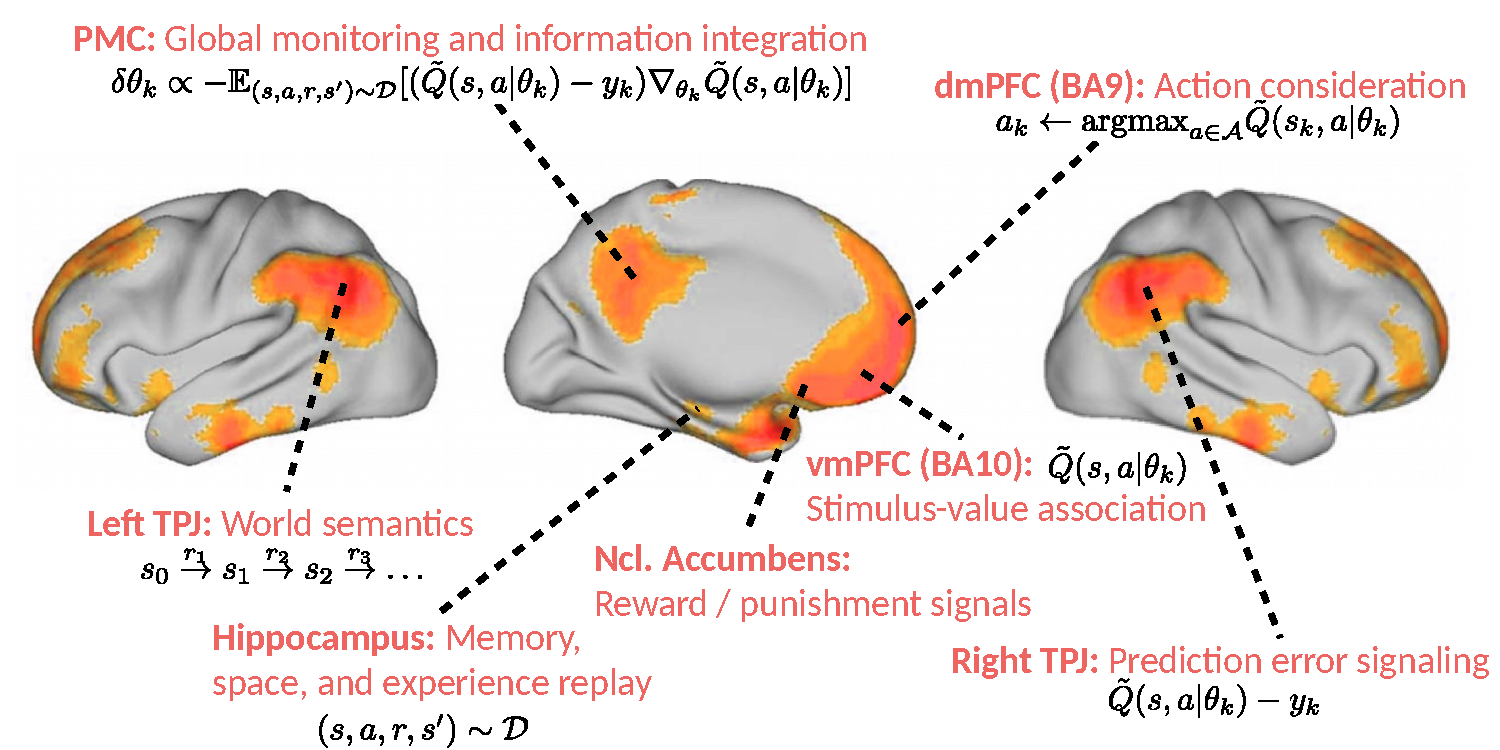
\includegraphics[width=.9\linewidth]{neurobiological_and_rl_overview_DMN.pdf}
  \caption{\textbf{Default mode network:
  neurobiological implementation of reinforcement learning.}
  Overview of how the constituent nodes of the DMN (refer to section \ref{sec:nodes}) may
  map onto computational components necessary for an RL agent.}
  \label{fig:rl_process_chart}
\end{figure}


The HC may contribute to generation of
perturbed action-transition-state-reward samples
as batches of pseudo-experience
(i.e., imagined, hypothesized, and recalled mental scenarios).
The small variations in these experience samplings allow searching
a larger space of model parameters and possible experiences.
Taken to its extreme, stochastic recombination of experience
building blocks can further optimize the behavior of the RL agent
by model learning from scenarios in the environment that the agent might
only very rarely or never encounter.
An explanation is thus offered for experiencing seemingly familiar situations that
a human has however never actually encountered (i.e., d\'{e}j\`{a} vu effect).
While such a situation may not have been experienced in the physical world,
the DMN may have previously stochastically generated, evaluated, and adapted to
such a randomly synthesized situation.
In the absence of environmental input and feedback
(e.g., mind-wandering or sleep),
mental scene construction allows for pseudo-experiencing possible
future scenarios and action outcomes.
Our formal account of DMN function
thus acknowledges the unavoidable stochasticity of
computation in neural systems \citep{faisal2008noise}.


From the perspective of a model-free RL agent,
\textit{prediction} in the human brain reduces to
generalization of
policy and value computations from sampled experiences to
successful action choices and reward predictions in future states.
As such,
plasticity in the DMN arises naturally.
If an agent behaving optimally in a certain environment moves
to new, yet unexperienced environment, reward prediction errors will
largely increase.
This feedback will lead to adaptation of policy considerations
and value estimations until the intelligent system converges to a
new steady state of optimal action decisions in a volatile world.



% \paragraph*{Some notes:}
% \begin{itemize}
%   \item Actions are continuous, whilst states are continuous.
%   \item The brain does backprop (see Hinton's recent talk at Stanford)
%   \item model weights $\theta^Q$ should correspond to connections between neurons
% \item humm, looks like such a knowledge would simply translate into constraints on the DqN weights $\theta^Q$ (... at least, part of such knowledge)
%   ok, gotta think about the model-free / model-based reconsiliation
% \end{itemize}


\begin{mdframed}
  \vspace{1em}
  \textbf{Box 2: Hypotheses for testing the MDP account of DMN function}
\begin{enumerate}
\item Experiment (Humans): We hypothesize a functional relationship between the DMN closely associated with the occurrence of stimulus-independent thoughts and the reward circuitry. During an iterative neuroeconomic two-player game, fMRI signals in the DMN could be used to predict reward-related signals in the nucleus accumbens across trials in a continuous learning paradigm. We expect that the more DMN activity is measured to be increased, supposedly the higher the tendency for stimulus-independent thoughts, and the more the fMRI signals in the reward circuits should be independent of the reward context
in the sensory environment.

\item Experiment (Humans): We hypothesize a functional dissociation between computations for behavioral policy versus adapting stimulus-value associations as these are conceivably implemented in different subsystems of the DMN. We first expect that fMRI signals in the right temporo-parietal junction can predict behavioral changes caused by adaptation in the action choice tendencies (policy matrix) related to non-value-related prediction error. Second, fMRI signals in the ventromedial prefrontal cortex should predict behavioral changes caused by adaptation in value estimation (value matrix) due to reward-related stimulus-value association. We finally predict that fMRI signals in the posteromedial cortex, as a potential global information integrator, is able to predict shifts in overt behavior based on previous adaptations in policy or value estimation.

\item Experiment (Animals): We hypothesize that experience replay for browsing problem solutions subserved by the DMN is necessary for choice behavior in mice. Hippocampal single-cell recordings have shown that neural patterns during experimental choice behavior are reiterated during sleep and before make analogous choices in the future. Necessity of the DMN, in addition to the hippocampus, for “mind-searching” actions during choice behavior can be demonstrated by causal disruption of DMN regions, such as circumscribed brain lesion or optogenetic intervention in the inferior parietal and prefrontal cortices.

\item Experiment (Humans): We hypotherize that time horizon should be modulated by different factors such as age, stress, and impulsivity. Using a temporal discounting task, we can measure how the time horizon could be affected at the behavioral level, and then trace back its potential representation at the neural level. Experimental design can be between groups (by age or with a impulsive population like chronic gamblers or drug addicts), or within group using a stress. 

% To exam-ine this question, Fellows and Farah (2005) investigated the effects of dorsolateral frontal (DLF) and ventromedial frontal (VMF) lobe damage on two aspects of temporal foresight—namely, temporal discounting and the futuretime perspective (measuredby an adaptation of Wallace’s [1956] list of future life events).

\item Experiment (Animals): how synaptic epigenesis between DMN nodes can form a neural correlate of the policy matrix update? % Simulations:

\end{enumerate}
\end{mdframed}


\begin{figure}[!h]
  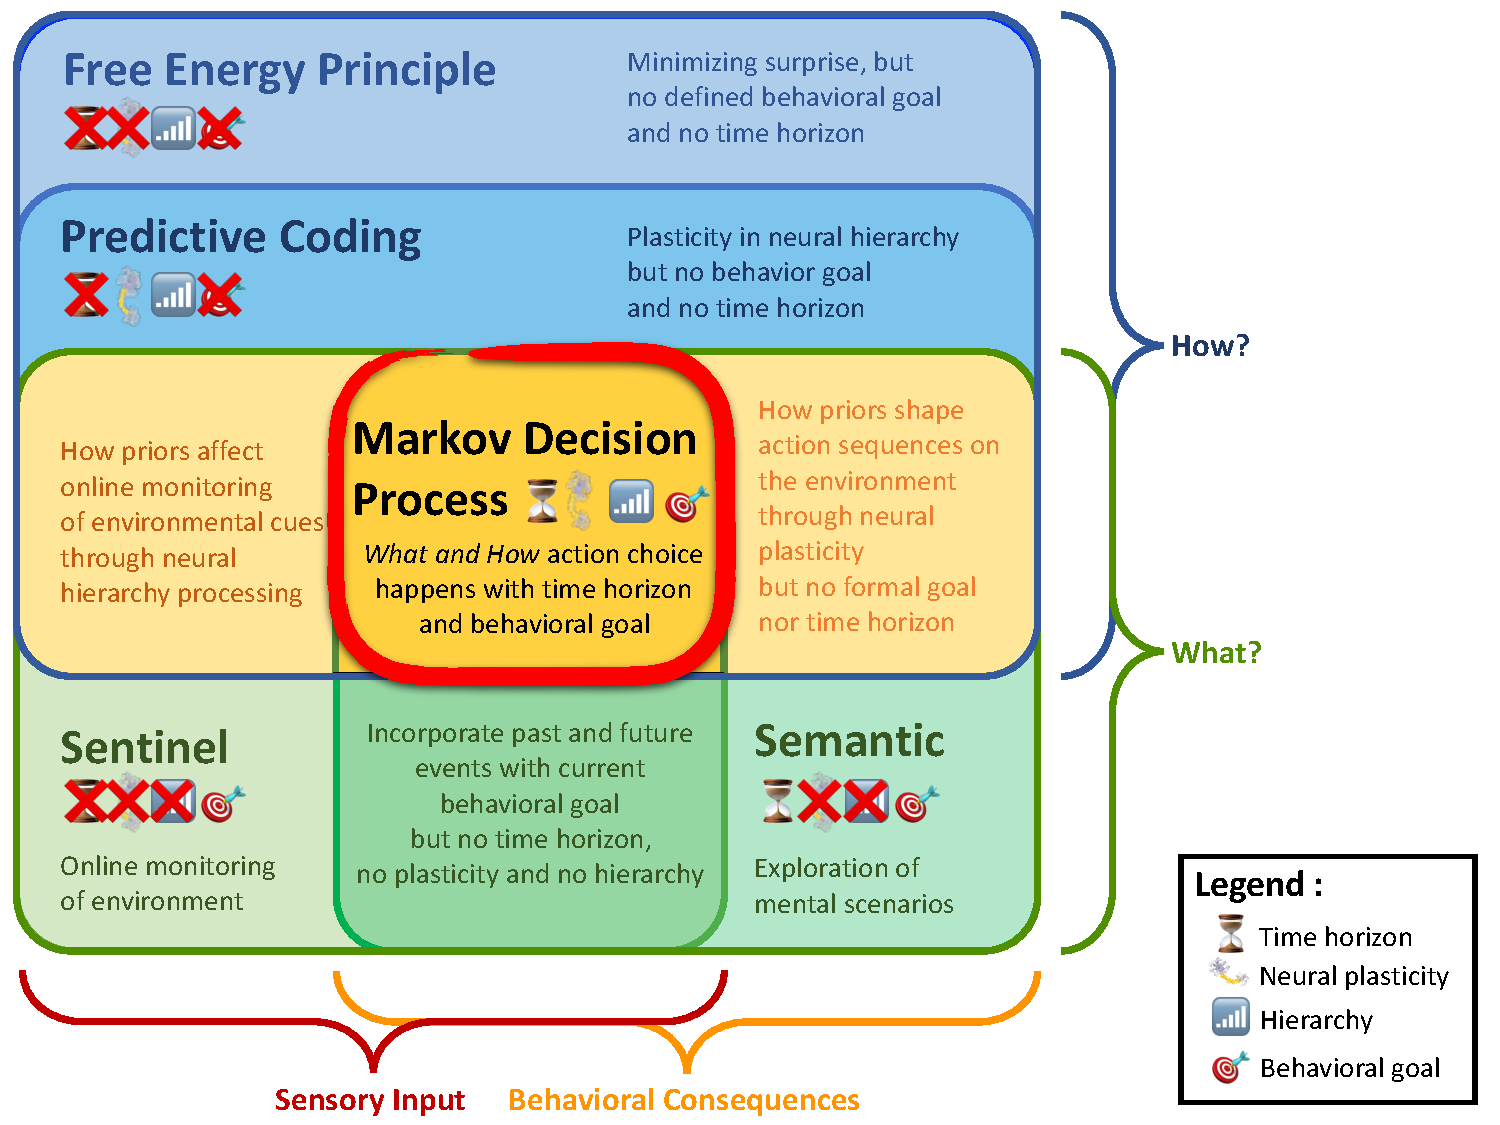
\includegraphics[width=1\linewidth]{VennDiagram-2017-09-08.pdf}
  \caption{\textbf{Situating Markov Decision Processes among other accounts of default mode function}
  This Venn diagram summarizes the relationship between four existing explanations of the functional role of the DMN and our present account. Viewing empirical findings in the DMN from the MDP viewpoint incorporates important aspects of the free energy principle, predictive coding, sentinal hypothesis, and semantic hypothesis.
  The MDP account may reconcile several strengths of these functional accounts in a process model that simultaneously acknowledges environmental input and behavioral choices as well as the computational and algorithmic properties (How? and What?) underlying higher-order control of the organism.}
  \label{fig:VennDiagram}
\end{figure}

\section{Relation to existing accounts}

\subsection{Predictive coding hypothesis}
Predictive coding mechanisms
\citep{clark2013whatever, friston2008hierarchical}
are a frequently evoked idea in the context of default mode function
\citep{bar2007}.
Cortical responses are explained as
emerging from continuous functional interaction between
higher and lower levels of the neural processing hierarchy.
Feed-forward sensory processing is constantly calibrated by
top-down modulation from more multi-sensory and associative brain regions
further away from primary sensory cortical regions.
The dynamic interplay between cortical processing levels
may enable learning about aspects of the world by reconciling
gaps between fresh sensory input and expectations computed
based on stored prior information.
At each stage of neural processing,
an internally generated prediction of aspects of environmental sensations is
directly compared against the actual environmental input.
A prediction error at one of the processing levels
induces plasticity changes of neuronal projections
(i.e., adapting model parameters)
to allow for gradually improved future prediction of the environment.
In this way,
the predictive coding hypothesis offers explanations for
the constructive, non-deterministic nature of sensory perception
\citep{friston2010free, buzsaki2006rhythms} and
the intimate relation of motor action to sensory expectations
\citep{wolpert1995internal, kording2004bayesian}.
Contextual integration of sensorimotor perception-action cycles
may be maintained by top-down modulation
using a-priori information about the environment.



In short, predictive coding processes
conceptualize updates of the internal representation of the environment
to best accommodate and prepare the organism
for processing the constant influx of sensory stimulation and
performing action on the environment.
There are hence a number of common properties
between the predictive coding account
and the proposed formal account of DMN function based on MDPs.
Importantly,
a generative model of how perceived sensory cues arise in the
world would be incorporated into
the current neuronal wiring.
Further,
both functional accounts are supported by
neuroscientific evidence that suggest
the human brain to be a ``statistical organ'' \citep{friston2014phantastic}
with the biological purpose to
generalize from the past to new experiences.
Neuroanatomically, axonal
back projections indeed outnumber by far the axonal input projections
existing in the monkey and probably also human brain
\citep{salin1995corticocortical}.
These many and diverse modulatory influences
from higher onto downstream cortical areas
can inject prior knowledge
at every stage of processing environmental information.
%
Moreover,
both accounts provide a parsimonious explanation for why the
human brain's processing load devoted to incoming information decreases
when the environment becomes predictable.
This is because the internal generative
model only requires updates after discrepancies have occurred between
environmental reality and its internally reinstantiated representation.
Increased computation resources are however allocated
when unknown stimuli or
unexpected events are encountered by the organism.
The predictive coding and MDP account hence
naturally evoke a mechanism of brain plasticity in that
neuronal wiring gets increasingly adapted
when faced by unanticipated environmental challenges.


While sensory experience is a constructive process from both views,
the predictive coding account frames
sensory perception of the external world
as a generative experience due to the modulatory top-down influence at
various stages of sensory input processing.
This generative top-down design is replaced in our MDP view of the DMN
by a sequential decision-making framework.
Further,
the hierarchical processing aspect from predictive coding
is re-expressed in our account in the form of
nested prediction of probable upcoming actions, states, and outcomes.
While both accounts capture the consequences of action,
the predictive coding account is typically explained without
explicit parameterization of the agent's time horizon and
has a tendency to be presented as emphasizing prediction about the
immediate future.
In the present account, the horizon of that
look into the future is made explicit in the $\gamma$ parameter
of the Bellman equation.
% \item \suggestremove{Mismatch negativity of PC is immanent in reward prediction error
% by the difference between actually predicted reward of an action given
% a state and the reward predicted by non-linear regression with graded
% discounting of future rewards.}
Finally,
the process of adapting the neuronal connections
for improved top-down modulation
takes the concrete form of stochastic gradient computation and
back-propagation in our MDP implementation.
It is however important to note that
the neurobiological plausibility of
the back-propagation procedure is controversial
\citep{goodfellow2016deep}.


In sum,
recasting DMN function in terms of MDPs therefore naturally incorporates
a majority of aspects from the prediction coding hypothesis.
The present MDP account of DMN function may therefore
serve as a concrete implementation of
predictive coding ideas from cognitive neuroscience.
MDPs have the advantage of exposing an explicit
mechanism for the horizon of future considerations and for
how the internal representation of the world is updated,
as well as
why certain predictions may be more relevant to the agent than others.




\subsection{Semantic hypothesis}
Another frequently proposed cognitive account to explain DMN function revolves
around forming logical associations and abstract analogies between
experiences and conceptual knowledge derived from past behavior
\citep{bar2007proactive, binder1999conceptual, constantinescu2016organizing}.
Analogies might naturally tie incoming new sensory stimuli to
explicit world knowledge (i.e., semantics)
\citep{bar2009proactive}.
The encoding of complex environmental features could thus be facilitated
by association to known similar states.
%
Going beyond isolated meaning and concepts extracted from the world,
semantic building blocks may need to get recombined to enable
mental imagery of non-existing scenarios.
As such, semantic knowledge would be a prerequisite for optimizing behavior
by constantly simulating possible future scenarios
\citep{boyer2008evolutionary, binder2011neurobiology}.
Such cognitive processes can afford
the internal construction and elaboration of necessary information
that is not presented in the surrounding sensory environment
by recombining building blocks of
concept knowledge and episodic memories
\citep{hassabis2009construction}.
Indeed, in aging humans, remembering the past and imagining the future
equally decreased in the level of detail and were associated with
concurrent deficits in forming and integrating relationships between
items \citep{addis2008age, spreng2006temporal}.
Further,
% a constructive account can explain the reciprocal relationship
% between an egocentric first person perspective and
% an allocentric bird’s eye perspective immersed in
% self-reflection, semantic associations, and autobiographical memories.
% %
% Cognitive aspects of egocentric-allocentric switching
episodic memory, language, problem solving,
planning, estimating others' thoughts, and spatial navigation
represent neural processes that are likely to
build on abstract world knowledge and logical associations
for integrating the constituent elements in rich and coherent mental scenes
\citep{schacter2007remembering}.
Such scene construction processes could contribute to interpreting the
present and foretelling the future.
Further,
mental scene construction has been proposed
to imply a distinction between
engagement in the sensory environment
and internally generated mind-wandering
\citep{buckner2007self}.
These investigators stated that
``A computational model [...] will probably require a form of
regulation by which perception of the current world is suppressed
while simulation of possible alternatives are constructed,
followed by a return to perception of the present.''.
% The semantic hypothesis is for instance supported by evidence in animals that
% could learn a \textit{cognitive map of the environment}
% and exploit it later for other means \citep{tolman1948cognitive}.


In comparison,
both the semantic hypothesis and the present formal account based on MDPs
expose mechanisms of how action considerations could be mentally explored.
In both accounts,
there is also no reason to assume that predictions of various
levels of complexity, abstraction, timescale, and purpose
rely on mechanisms that are qualitatively different. This concurs with
DMN activity increases across time, space, and content domains
demonstrated in many neuroimaging studies
\citep{spreng2009common, laird2009, bzdok2012morality, binder2009}.
Further, the semantic hypothesis
and MDP account provide explanations why HC damage does
not only impair recalling memories, but also hypothetical and future
thinking \citep{hassabis2007patients}.
While both semantic hypothesis and
our formal account propose memory-based internally
generated information for probabilistic mental models of action outcomes,
MDPs render explicit the grounds on which an action is
eventually chosen, namely, the estimated cumulative reward.
In contrast to many versions of the semantic hypothesis,
the MDPs naturally integrate the egocentric view
(more related to current action, state, and reward) and the
world view (more related to past and future actions, states, and rewards)
on the world in a same optimization problem.
Finally,
the semantic account of DMN function does not offer
a mechanistic explanation \textit{how}
explicit world knowledge and semantic analogies thereof
lead to prediction of future actions and states.
The semantic hypothesis does also not explain why memory recall
for scene construction in humans is typically fragmentary and noisy
instead of accurate and reliable.
In contrast to existing accounts on semantics and
mental scene construction, the random and creative aspects of DMN function
are explained in MDPs by the advantages of stochastic optimization.
Our MDP account provides an algorithmic explanation in that
stochasticity of the parameter space exploration
by MCMC approximation achieves better fine-tuning of the
action policies and estimation of expected reward outcomes.
That is, the purposeful stochasticity of policy and value estimation
in MDPs provides a candidate explanation for why humans
have evolved imperfect noisy memories
as the more advantageous adaptation.
In sum, mental scene construction according to the semantic
account is lacking an explicit time and incentive model,
both of which are integral parts of the MDP interpretation of DMN function.



\subsection{Sentinel hypothesis}
The DMN regions have been associated with processing the
experienced or expected relevance of environment cues
\citep{montague2006imaging}.
Processing self-relevant information was perhaps the first
cognitive account that was proposed for DMN function
\citep{gusnard2001medial, raichle2001pnas}.
Since then,
many investigators have speculated that neural activity in the DMN
may reflect the brain's continuous tracking of
relevance in the environment, such as spotting predators,
as an advantageous evolutionary adaptation \citep{randy2008, hahn2007cingulate}.
According to this cognitive account, the human brain's baseline maintains
a ``radar'' function to
detect subjectively relevant cues and unexpected events in the environment.
Propositions of a sentinel function to underlie DMN activity
have however seldom detailed
the mechanisms of
how attention and memory resources are exactly reallocated when
encountering a self-relevant environmental stimulus.
However,
in the present MDP account,
promising action trajectories
are recursively explored by the human DMN. Conversely,
certain branches of candidate action trajectories
are detected to be less worthy to become mentally explored.
This mechanism, expressed by the Bellman equation,
directly implies stratified allocation of attention and working memory load
over relevant cues and events in the environment.
%
Further,
our account provides a parsimonious explanation for
the consistently observed DMN implication
in certain goal-directed experimental tasks and
in task-unconstrained mind-wandering \citep{smith2009, bzdok2016formal}.
Both environment-detached and environment-engaged
cognitive processes may entail DMN recruitment
if real or imagined experience is processed, manipulated, and
used for predictions.
During tasks,
the policy and value estimates may be
updated to optimize especially short-term action.
At rest, these parameter updates may
improve especially mid- and long-term action.
This horizon of the agent
is expressed in the $\gamma$ parameter in the MDP account.
We thus provide answers for the currently unsettled question why the involvement
of the same neurobiological brain circuit (i.e., DMN) has been documented
for specific task performances and baseline house-keeping functions.



In particular,
environmental stimuli are especially important for humans are frequently of
social nature. This is not surprising
given that
the complexity of the social systems
is likely to be a human-defining property
\citep{tomasello2009cultural}.
According to the ``social brain hypothesis'',
the human brain has especially been shaped for
forming and maintaining increasingly complex
social systems,
which allows solving ecological problems by means of social relationships
\citep{whiten1988machiavellian}.
Indeed, social topics amounted to roughly
two thirds of human everyday communication \citep{dunbar1997human},
while
mind-wandering at daytime and dreams during sleep
are rich in stories about people and
the complex relationships between them.
%
In line with this, the DMN was argued to be specialized in
continuous processing of social information as a
physiological baseline of human brain function
\citep{schilbach2008minds}. This view was later challenged by observing
analogues of the DMN in monkeys \citep{mantini2011default},
cats \citep{popa2009contrasting},
and rats \citep{lu2012rat}, three species with
social-cognitive capacities that are supposedly less advanced than in humans.


Further,
the principal connectivity gradient in the cortex appears to be greatly expanded in humans compared to monkeys, suggesting a phylogenetically conserved axis of cortical expansion with the DMN emerging at the extreme end in humans \citep{margulies_situating_2016}. Neurocomputational models of dyadic whole-brain dynamics
demonstrated how the human connectivity topology, on top of facilitating processing at the intra-individual level, can explain our propensity to coordinate through sensorimotor loops with others at the inter-individual level \citep{dumas_anatomical_2012}.
The DMN is moreover largely overlapping with neural networks associated with higher level social cognition \citep{schilbach_introspective_2012}. For instance, the vmPFC,
PMC, and RTPJ
together play a key role in bridging the gap between self and other by
integrating low-level embodied processes within higher level inference-based mentalizing \citep{lombardo_shared_2009}.


Rather than functional specificity for processing social information,
the present MDP account can parsimoniously incorporate
the dominance of social content in
human mental activity
as high value function estimates for information about humans
\citep{baker2009action, kampe2001psychology, krienen2010clan}.
The DMN may thus modulate reward processing
in the human agent in a way that prioritizes
appraisal of and action towards social contexts,
without excluding relevance of environmental cues of the physical world.
In sum,
our account on the DMN directly implies
its previously proposed ``sentinel'' function
of monitoring the environment for self-relevant information
in general and
inherently accommodates the importance of social environmental cues
as a special case.


\subsection{The free-energy principle and active inference}
% INTRO
According to theories of the \textit{free-energy principle} (FEP) and
\textit{active inference} \citep{friston2010free, fristonAIorRL} (see also \citep{dayan1995helmholtz}),
the brain corresponds to
a biomechanical reasoning engine. It is
dedicated to minimizing the long-term average of surprise: the log-likelihood of the observed sensory input --more precisely, an upper bound thereof-- \textit{relative} to the expectations about the external world derived from internal representations. The brain
would continuously generate hypothetical explanations of the world
and predict its sensory input $\bf{x}$ (analogous to the state-action $(s, a)$ pair in an MDP
framework).
% Precursors of this interpretation can be traced back to Dayan and colleagues \citep{dayan1995helmholtz}
% who introduced the \textit{Helmholtz machine}, a hierarchical factorial directional deep belief network. According to the FEP account,
% the goal of the brain is to optimize over a generative model $G$ of sensations: to iteratively
% modify its internal representation $p_G(\z|\x)$ of objects in the world, their interactions and dynamics. The model then allows
% to minimize surprise when these representations are confronted with sensory input $\x$ during action-perception cycles (i.e., the \textit{generative} model).
% The FEP also proposes a companion model called the \textit{recognition} model $p_R(\z|\x)$,
% which works in tandem with the generative model to accomplish approximate inference. Put differently, the recognition model dreams imaginary worlds $\z$,
% while the generative model tries to produce sensory sensations $\x \sim p_G(\x|\z)$ which match these
% imagined mental scenarios.
However, surprise is challenging to optimize numerically
because we need to sum over all hidden causes $\z$ of the sensations (an intractable problem).
Instead, FEP therefore minimizes an upper-bound on surprise given by

\begin{equation}
  \begin{split}
    \text{generative surprise } &:= -\log(p_G(\x)) = F_G(\x) \\
    &=\underbrace{F^R_G(\x)}_{\text{accuracy}} - \underbrace{\operatorname{{KL}}(p_R(\z|\x) \| p_G(\z|\x))}_{\text{complexity}} \\
    &\le F^R_G(\x),
    \text{ with equality if }p_R(\z|\x) = p_G(\z|\x)\text{ for all } \z.
  \end{split}
\end{equation}
where
\begin{equation}
  F_G^R(\x) := \langle -\log(p_G(\z, \x))\rangle_{p_R(\z|\x)} - \mathcal H(p_R(\z|\x))
\end{equation}
is the \textit{free energy}.
Here, the angular brackets denote the \textit{expectation} of the joint negative log-likelihood $-\log(p_G(\z, \x))$ w.r.t the recognition density $p_R(\z|\x)$, $\mathcal H$ is the \textit{entropy} functional defined by $\mathcal H(p) := -\sum_{\z}p(\z)\log(p(\z)$, while $\operatorname{KL}(.\|.)$ is the usual \textit{Kullback-Leibler (KL) divergence} (also known as \textit{relative entropy}) defined by $\operatorname{KL}(p\|q) := \sum_{z}p(\z)\log(p(\z)/q(\z)) \ge 0$,
which is a measure of how different two probability distributions are. In this framework, the goal of the agent is then to iteratively refine the generative model $p_G$ and the recognition model $p_R$ (i.e two Bayesian belief nets) so as to minimize the free energy $F_G^R(\x)$ over sensory input $\x$.

Importantly, one notes that $F^R_G(x)$ is low just in case:
\begin{itemize}
\item  $p_R(\z|\x)$ puts a lot of mass on configurations $(\z,\x)$ which are $p_G$-likely, % (i.e the sensation $\x$ is likely caused by $\z$)
  \textbf{and}
\item $p_R(\z|\x)$ is as uniform as possible (i.e have high entropy), so as not to concentrate
  all its mass on a small subset of possible causes for the sensation $\x$.
  \end{itemize}
% The optimization procedure proposed by the authors derives from the \textit{wake-sleep algorithm} \citep{dayan1995helmholtz}.
% \begin{figure}[!tb]
%   \centering
%   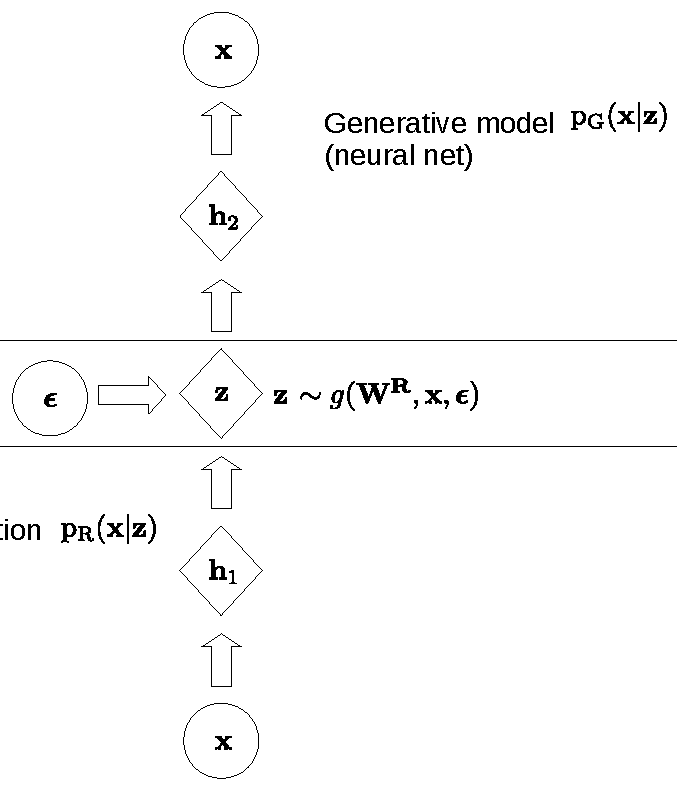
\includegraphics[width=.8\linewidth]{vae.pdf}
%   \caption{Variational autoencoders...}
%   \label{fig:vae}
% \end{figure}


% CRITICISM
% \paragraph{Main criticisms.}
Despite its popularity, criticism against the FEP has arisen over the years,
some of which is outlined in the following.
The main algorithm for minimizing free energy $F_G^R(\x)$ is the \textit{wake-sleep algorithm}
\citep{dayan1995helmholtz}. As P. Dayan and G. Hinton themselves noted,
a crucial drawback of the wake-sleep algorithm (and therefore of theories like the FEP \citep{friston2010free} based on it) is that it involves a pair
of forward (generation) and backward (recognition) models $p_G$ and $p_R$ respectively that
together do not correspond to optimization of (a bound of) the marginal likelihood,
because KL divergence is not symmetric in its arguments.
The brain is therefore unlikely to implement the wake-sleep algorithm or a variant thereof.

The recent theory of
\textit{variational auto-encoders} (VAEs) \citep{kingma2013auto} might provide an efficient alternative to the wake-sleep algorithm. VAEs
overcome a number of the technical limits of the wake-sleep algorithm
by using a reparametrization maneuver, which makes it possible to do differential calculus on random sampling procedures without exploding variance. As a result, unlike the wake-sleep algorithm
for minimizing free energy, VAEs can be efficiently trained via back-propagation of prediction errors.

\begin{wrapfigure}{r}{.37\linewidth}
  \centering
  
\includegraphics[width=1.\linewidth]{darkroom_resized.png}
  \caption{\textbf{The dark room experiment.} An intelligent agent situated
  in a light-deprived closed space is used
  as a thought experiment for the complete absence
  of external sensory input.
  % The free-energy principle theory paradoxally predicts that such an agent would remain quietly in this room, such it perfectly predict all sensory input from such an environment.
  % However such behavior is not observed in humans or any animals: the agent would strive to leave such an environment in search of more ``interesting'' worlds.
  }
  \label{fig:darkroom}
\end{wrapfigure}

On another front, since theories based on the FEP \citep{friston2010free,fristonAIorRL}
conceptualize ongoing behavior
in an organism to be geared towards the surprise-minimizing goal,
an organism entering a dark room
% \footnote{\textit{Dark} is used here as an allegory to indicate the complete absence of any \textit{external} sensory input.}
(Fig. \ref{fig:darkroom}) would strive to remain in this location
because its sensory inputs are perfectly predictable
given the environmental state \citep{darkroom2012}.
However, such a behavioral tendency is
seldom observed in animals or humans in the real world: In a dark room,
intelligent agents would search for light sources to \textit{explore}
the surroundings or leave the exit the room.
Defenders of the FEP have retorted by advancing the ``full package'' \citep{darkroom2012}:
FEP is proposed to be multi-scale and there would be a meta-scale at which the organism would
be \textit{surprised} by such a \textit{lack of surprise}. According to this argument, a dark room would paradoxically correspond to a state of particularly high surprise.
Driven by surprise-minimization objective, the FEP agent would eventually bootstrap itself out of such saddle points to explore more interesting parts of the environment.
% Recourse to this argument is equivalent to invoking a \textit{halting oracle}\citep{haltingoracle}, an arbitrarily powerful machine which can solve the \textit{halting problem} (an arbitrarily difficult computational problem which cannot be solved under any reasonable \textit{model of computation}, not even in principle!). But this is problematic as it sucks up the problem (that of decision-making and active agency) the theory intends to elude in the first place.
In contrast, an organism operating under our RL-based theory would inevitably
identify the sensory-stimulus-deprived room as a local minimum. Indeed, hippocampal experience replay (see \ref{sec:self}) would serve to sample memories or fantasies of alternative situations
with reward structure. Such artificially generated \textit{internal} sensory input
subserved by the DMN can entice the organism to explore the room,
for instance by looking for and using the light switch or simply finding the room exit.

% \paragraph{Links between FEP and RL.}
We note that FEP and active inference can be reframed in terms of
our model-free RL framework.
This becomes possible by recasting the Q-value function (i.e expected long-term reward) maximized by the DMN to
correspond to negative surprise,
that is, the log-likehood of current sensory priors
the agent has about the world. More explicitly, this corresponds to using free-energy as a Q-value approximator for the MDP, i.e

\begin{eqnarray*}
  -Q \approx \underbrace{F^R_G(\x)}_{\text{negative free energy}} \approx \underbrace{-\log (p_G)}_{\text{FEP generative surprise}}.
    \end{eqnarray*}
% \paragraph{Comparison to our proposed theory.}
% On the surface, a common point between the FEP and our proposed RL-based framework
%   is placing the minimization of a surprise signal at the core of brain function.
%   Indeed in RL, surprise minimization is subsumed  by accurate prediction of
%   rewarding outcomes in the future. A ``free-energy'' agent is barely a biomechanical machine which has the tendency to resist undesired phase-transitions
%   \citep{friston2010free,fristonAIorRL,ortega2013thermodynamics}.
Such a surprise-guided reinforcement learning scheme has previously been advocated
under the equivalent framework of energy-based reinforcement-learning
% \footnote{These methods assume that the posterior distribution  of the hidden states $\z$ given the visible states $\x$ factorizes, leading to so-called RBMs --\textit{Restricted Boltzmann Machines}. One notes, that even with these simplifications, such a model can be very hard to train.}
~\citep{sallans2004,elfwing2016free} and information compression \citep{schmidhuber2010,mohamed2015}.
Nevertheless, minimization of surprise quantities alone
may be insufficient to explain the diversity of behaviors observed in humans and other intelligent animals.
% The dark-room experiment, for example, provides a formidable argument against in favor of the insufficiency of the FEP and active inference theories to explain intelligent behavior in humans: when a human is put in a dark room, they don't just sit down in a corner forever, what would be the FEP-optimal thing to do; they actively search for the light switch, and start exploring the depths of the room, possibly looking for food or the way out!

% Friston's critic of RL \citep{fristonAIorRL} (he proposes ``active inference''): "This equation (equation 18) comes from the theory of dynamic programming,
% pioneered in the 1950s by Richard Bellman and colleagues [2]. To
% optimise control a~pð Þ x~ under this formulation, we have to: (i)
% assume the hidden states are available to the agent and (ii) solve
% Equation 18 for the value-function. Solving for the value-function
% is a non-trivial problem and usually involves backwards induction
% or some approximation scheme like reinforcement learning [4–6].
% The free-energy formulation circumvents these problems by
% prescribing the policy in terms of free-energy, which encodes
% optimal control (Equation 6)"

% The following critics can be made:
% \begin{itemize}
%   \item
%     As noted by Dayan et al. (\textit{Variants of Helmholtz machines}), the inter-neuronal intra-layer independence assumption which is at the center of the HM becomes severely problematic as it is agnostic to the known organization of cortical layers...
%   \item A drawback of the wake-sleep algorithm is that it requires a concurrent models (generative and recognitiion), which together do not correspond to optimization of (a bound of) the marginal likelihood (because of the incorrect KL used therein, etc.).
%   \item Also, note that the wake-sleep algorithm doesn't do backprop! This is due to
%     technical difficulty in getting derivatives of loss function w.r.t
%     recognition weights $\W^R$).
%   \item This difficulty was removed in the 2010s by \citep{kingma2013auto}, an other groups, via a ``reparametrization trick''.
%   \end{itemize}

% \textbf{XXX: integrate aspects from Friston2014(Dropbox) on active inference}

\section{Conclusion}
Which brain function could be important enough
for the existence and survival of the human species
to justify constantly high energy costs?
MDPs motivate an attractive
formal account of how the human association cortex
might implement multi-sensory representation and control of the environment to
optimize the organism's interaction with the world.
% by obtaining reward and avoiding pain.
This idealized process model explains
a number of previous experimental observations in the
DMN by simple but non-trivial mechanisms.
%
From the view of a Markovian sequential decision process,
human behavior unfolds by integrating action outcomes from policy matrix (mapping from states to actions which maximize expected cumulative reward; see subsection \ref{sec:policymat})
% stored past events
and extrapolation to
upcoming events for guiding action choice in the present context.
MDPs also provide a mathematical formalism how
opportunity in the environment can be recursively exploited
when confronted with challenging decisions.
%
This functional interpretation may well be compatible with the DMN's
poorly understood involvement across
autobiographical memory recall, problem solving,
abstract reasoning, social cognition,
as well as delay discounting and self-related prospection.
Improvement of the internal world representation
by injecting stochasticity into the recall of past
actions and the estimation of action outcomes may explain why
highly accurate memories have been disfavored in human evolution
and why human creativity might be adaptive.



It is an important feature of the proposed artificial intelligence perspective
on DMN biology that it is practically computable and
yields falsifiable neuroscientific hypotheses.
%
Neuroscience experiments could be designed that operationalize
the set of action, value, and state variables that govern
the behavior of intelligent RL agents.
%
At the least, we propose an alternative vocabulary to
describe, contextualize, and interpret experimental findings in neuroscience studies
on the DMN.
%
Ultimately,
DMN activity may instantiate a holistic integration
ranging from real experience over purposeful dreams to anticipated futures
for continued refinement of the organism's fate. Indeed, a major hurdle in explaining DMN activity from brain-imaging studies has been its very similar engagement across time scales: thinking about the past (e.g., autobiographical memory), thinking about hypothetical presents (e.g., dreams during sleep or daytime mind-wandering), and thinking about future scenarios (e.g., prospection or delay discounting). The MDP account of DMN function offers a natural integration of these a-priori diverging mental processes into a common framework. % It is this feature of our functional view that we underline in the referred sentence.




% \paragraph{Acknowledgment.}
% {\small The research leading to these results has received funding from the
% European Union Seventh Framework Programme (FP7/2007-2013)
% under grant agreement no. 604102 (Human Brain Project).
% Further support was received from
% the German National Academic Foundation (D.B.).
% }


\small
% \bibliographystyle{splncs03}
% \bibliographystyle{natbib}
\bibliographystyle{plainnat}
\bibliography{refs}


% \appendix
% 
% \begin{remark}
%   Given a system $(\mathcal S, \mathcal A, r, p, \mu)$ satisfying all the axioms for an MDP
%   except the Markov property, we can always transform it into an MDP by considering a compounded
%   version of the states
%   $$S_t \leftarrow (S_0,A_0,R_0,S_1,A_1,S_2\ldots,S_t,A_{t-1},R_{t-1},S_{t})$$ made of the system's
%   history up to an including time $t$.
% \end{remark}
% 
% \section{More on RL in the brain}
% \subsection{Does hippocampal replay equal inverse reinforcement-learning?}
% %\begin{mdframed}
%   Given the trace $s_0,a_0,s_1,\ldots,$ of an optimal agent's strategy $\pi^*$ in
%   an MDP (called a \textit{teacher's demonstration}), can we figure out what is the
%   (instantaneous) reward function $r: \mathcal S \times \mathcal \mathcal A
%   \rightarrow \mathbb R$ that the agent is optimizing over a prescribed class of reward functions
%   (e.g., linear rewards $r(s,a) \equiv \theta^T\phi(s,a)$)?
%   For instance, given traces of motor actions from an adult to grab a cup on a table,
%   can an observing child figure out what ``langragian'' functional is being minimized by the former?
%   How? Can they reproduce this optimal behavior?
% %\end{mdframed}
% Such questions are of course pertinent to our decision-making theory for the DMN.
% In the general artificial case, the problem has been extensively studied and partially solved by
% \citep{abbeel2004}. They are also been rigorously studied in general optimal control literature under the name
% ``inverse optimal control'', but in model-based certain (where the physical dynamics are known, etc.)...
% 
% IRL is is suited for problems in which it's hard to define what the reward function could be
% (e.g.,  car-driving, drone maneuvering, etc.) ...
% 
% \section{Free-energy principles!}
% The so-called free-energy principle in its present form (including notions like ``generative density'', ``recognition density'', etc.) can be traced back to works of Dayan \& Hinton \citep{dayan1995helmholtz} in which they introduced the so-called \textit{Helmholtz machine}, a hierarchical factorial directional deep belief-net (DBN).
% In this subsection, we will develop from first-principles, the bare-bones minimalistic ideas needed to build a free-energy principle for general decision-making. This ideas were first developed by Hinton et al. in the early 90s in building their Helmholtz machine. Theories like Friston's free-energy principle and active-inference will then emerge as particular instances of this general framework, with particular design choises. For instance, the Friston theory axiomatizes that the brain uses a (problematic, as it implicitly assumes that posterior of each hidden unit is factorial) wake-sleep algorithm to train the underlying Helmholtz machine, etc.
% 
% % \begin{mdframed}
% %   Though our presentation of free-energy principles is thermodynamic in flavor, a completely equivalent
% %   information-theoretic formulation is of course possible, simply by exploiting the information-theoretic interpretation of entropy.
% % \end{mdframed}
% 
% \subsection{Helmholtz free-energy and the generative model}
% \begin{table}[H]
%   \begin{tabular}{p{2cm}|p{11cm}}
%          \hline
%          \textbf{symbol}    & \textbf{description}  \\ \hline
%          $\langle X\rangle_p$ & Expectation (a.k.a average, a.k.a mean value) of the
%          random quantity $X$ w.r.t to the probability density $p$, formally defined by $\langle E\rangle_p := \sum_{z}p(z)X(z)$.\\ \hline
%          $\mathcal H(p)$ & Information-theoretic entropy of a probability density $p$, formally defined by $\mathcal H(p) := -\sum_{z}p(z)\log(p(z))$,
%           with the usual convention $0 \log(0) := 0$.\\ \hline
%          $D_{KL}(q||p)$ & The Kullback-Leibler divergence between the probability densities $q$ and $p$ respectively, formally defined by $D_{KL}(q||p) := \sum_{z}q(z)\log(q(z)/p(z))$.\\ \hline
%              $\x$ & Observations. In Friston's free-energy principle this has a decomposition in to two terms: the brain's internal state $b$ and sensory inputs $s$, i.e., $\x = (s, b).$ \\ \hline
%              $\z$ & Hidden variables. This should be understood as the unobservable states of the external environment (to which the brain is trying to adapt by learning).\\ \hline
%              $p_G(.|\x)$ & Generative density for ...\\ \hline
%          $p_R(.|\x)$ & Recognition density for ... Does some kind of predictive coding (?).\\ \hline
%          $F_G(\x)$ & Helmholtz free-energy for a model $p_G$ of generating the observation $\x$. This measures the surprise incured upon observing $\x$ generated by the model $G$.\\ \hline
%          $F^R_G(\x)$ & Variational Helmholtz free-energy from model $G$
%           to $R$.  Note that $F^G_G = F_G$.\\ \hline
%   \end{tabular}
%   \caption{Table of notations.}
% \end{table}
% Our starting point will be to build an approximation $p_G$ for the true density $p$ of the observations, so that this approximate density corresponds to the partition function of thermodynamic system. So,
% \begin{eqnarray}
%   \begin{split}
%     \text{generative surprise } &= -\log(p_G(\x)) = -\log(p_G(\x)) \times 1 = -\log(p_G(\x))\sum_{\z}p_G(\z |\x)\\
%     &= -\sum_{\z}p_G(\z, \x)\log(p_G(\x))
%     =-\sum_{\z}p_G(\z |\x)\log(p_G(\z, \x)/p_G(\z|\x))\\
%     &= \sum_{\z}p_G(\z |\x)\log(p_G(\z|\x))-\sum_{\z}p_G(\z |\x)\log  (p_G(\z, \x))\\
%     &= -\langle \log  (p_G(., \x)) \rangle_{p_G(. |\x)} - \mathcal H(p_G(. |\x))\\
%     &= \langle E_G(., \x) \rangle_{p_G(. |\x)} - \mathcal H(p_G(. |\x))
%   \end{split}
%   \label{eq:helm}
% \end{eqnarray}
% where $E_G(\z, \x)$ is the energy at \textit{macrostate} $\z$ of a fictive thermodynamic system defined by setting
% \begin{equation}
%   E_G(\z, \x) := -\log(p_G(\z, \x)),
%   \label{eq:gibbs}
% \end{equation}
% %% In the above, the variable $\z$ is a hidden variable, and can / should be interpreted as the unobservable state of the external world.
% The last quantity in \eqref{eq:helm} is nothing but \textit{Helmholtz free-energy} (at unit temperature!), defined formally by
% \begin{equation}
%   F_G(\x) := \langle E_G(., \x) \rangle_{p_G(. |\x)} - \mathcal H(p_G(. |\x)).
% \end{equation}
% %% , modelled as the physical system for which $p_G(\z|\x)$ dictates the occupation probabilities of macrostates $\z$
% Thus,
% \begin{fact}
%   Generative surprise and generative Helmholtz free-energy are different views on exactly the same object.
% \end{fact}
% 
% The goal of the brain is then to optimize over the generative model $G$: to iteratively or analytically modify the generative density $p_G(.|\x)$, so as to minimize surprise. It turns out that a direct attempt to attack this optimization problem by gradient descent on the free-energy $F_G(\x)$ is furtile: the parameter update steps are not ``very clean'', and require rather cumbersome and heavy computations. A workaround is then to introduce a second density $p_R(.|\x)$ called a \textit{recognition} density to work in tandem with the generative density $p_G(.|\x)$, as a trick for doing approximate inference. The former dreams / fantacizes whilst the latter tries to generate sensations which match these dreams! This primal-dual idea, first proposed in Hinton et al. 1995, is at the heart of the general free-energy principle that we will introduce shortly.
% 
% \subsection{Variational Helmholtz free-energy and the bottom-up recognition sub-model}
% In this subsection, we will present an insightful upper bound for the generative surprise (i.e., generate Helmholtz free-energy), called the \textit{variational} (Helmholtz) free-energy. As an avant-gout of what is to come shorty, let's just note that the well-known \textit{free-energy principle} is simply a workaround whereby the minimization surprise (intractable) is replaced with the  minimization a carefully chosen upper bound thereof.
% 
% Invoking \eqref{eq:gibbs} and applying Bayes rule, we get the Gibbs
% distribution
% \begin{equation}
%   p_G(\z|\x) = \frac{p_G(\z|\x)}{p_G(\x)} = \frac{\exp(-E_G(\z, \x))}{Z_G(\x)} = \frac{\exp(-E_G(\z, \x))}{Z_G(\x)},
% \end{equation}
% where $Z_G(\x) := \log(p_G(\x)) = \sum_{\z'}\exp(-E_G(\z',\x))$, the normalizing \textit{partition function} for the model \ref{eq:gibbs}.
% Whence, for any macrostate $\z$, we have $p_G(\x) = Z_G(\x) = \exp(-E_G(\z, \x)) / p_G(\z|\x)$, and so it holds that
% \begin{equation}
% F_G(\x)\overset{\eqref{eq:helm}}{=} -\log(p_G(\x)) = -\log(Z_G(\x)) = E_G(\z, \x) + \log(p_G(\z|\x)).
% \end{equation}
% Now, in the above equation, the LHS only depends on the generative model $G$ and the data point $\x$:
% it doesn't depend on the hidden variable $\z$, etc. So, taking expectations w.r.t an arbitrary
% density\footnote{conditioning in $p_R(.|\x)$ is because this density is selected from a world in which the sensory inputs and internal brain
%   state vector $\x$ is assumed already observed.} $p_R(.|\x)$ yields
% \begin{equation}
%   \begin{split}
%     F_G(\x) &= -\log(Z_G(\x)) = \langle E_G(., \x)\rangle_{p_R(.|\x)} + \sum_{\z}p_R(\z|\x)\log(p_G(\z|\x))\\
%     &= \langle E_G(., \x)\rangle_{p_R(.|\x)} - \mathcal H(p_R(.|\x)) - \sum_{\z}p_R(\z|\x)\log(p_R(\z|\x)/p_G(\z|\x))\\
%     &= F^R_G(\x) - D_{KL}(p_R(.|\x) || p_G(.|\x)),
%   \end{split}
%   \label{eq:fe}
% \end{equation}
% where $F^R_G(\x)$ is the \textit{variational} Helmholtz free-energy from $R$ to $G$ defined by
% \begin{equation}
%   F^R_G(\x) := \langle E_G(., \x)\rangle_{p_R(.|\x)} - \mathcal H(p_R(.|\x))
% \end{equation}
% and $D_{KL}(p_R(.|\x) || p_G(.|\x))$ is the Kullback-Leibler divergence between the $p_R(.|\x)$ and the generative density $p_G(.|\x)$. Note that $F^G_G = F_G$.
% 
% \subsection{A general free-energy principle}
% We can resume the situation as follows\footnote{Where we have used the fact that KL divergence is always nonnegative.}:
% \begin{mdframed}
% \begin{equation}
%   \begin{split}
%     \text{generative surprise } &:= -\log(p_G(\x)) = F_G(\x) \\
%     &=\underbrace{F^R_G(\x)}_{\text{accuracy}} - \underbrace{D_{KL}(p_R(.|\x) || p_G(.|\x))}_{\text{complexity}} \\
%     &\le F^R_G(\x),
%     \text{ with equality if }p_R(\z|\x) = p_G(\z|\x)\text{ for all } \z
%     \end{split}
% \end{equation}
% \end{mdframed}
% %% In fact, we have the following theorem
% %% \begin{theorem}
% %%   It holds that
% %%   $$
% %%   \text{Minimal generative surprise = minimal (Helmholtz) variational free-energy},$$
% %%   i.e
% %%   \begin{equation}
% %%     \min_{G}F_G(\x) = \min_{G,R}F^R_G(\x)
% %%     \end{equation}
% %% \end{theorem}
% 
% \subsection{Helmholtz machines and the wake-sleep algorithm}
% % \begin{mdframed}
%   \textbf{Assumption:} In both generative and recognition components of the network, there is conditional independence of  neurons in the same layer, given the data (i.e., input from lower more primitive layers). Precisely
% $$
% p_G(\z^{(l)}|\x) = \Pi_{k=1}^{h_l}p_G(\z_k^{(l)} | \x),\hspace{1cm}
% p_R(\z^{(l)}|\x) = \Pi_{k=1}^{h_l}p_R(\z_k^{(l)} |\x)
% $$
% % \end{mdframed}
% 
% \subsection{Friston's active-inference and agency}
% \label{sec:friston}
% This is nothing but an application of the Dayan's wake-sleep algorithm for training a Helmholtz machine model of the brain...
% 
% The following critics can be made:
% \begin{itemize}
%   \item
%     As noted by Dayan et al. (\textit{Variants of Helmholtz machines}), the inter-neuronal intra-layer independence assumption which is at the center of the HM becomes severely problematic as it is agnostic to the known organization of cortical layers...
%   \item A drawback of the wake-sleep algorithm is that it requires a concurrent models (generative and recognitiion), which together do not correspond to optimization of (a bound of) the marginal likelihood (because of the incorrect KL used therein, etc.).
%   \item Also, note that the wake-sleep algorithm doesn't do backprop! This is due to
%     technical difficulty in getting derivatives of loss function w.r.t
%     recognition weights $\W^R$).
%   \item This difficulty was removed in the 2010s by \citep{kingma2013auto}, an other groups, via a ``reparametrization trick''.
%     \end{itemize}
% 
% 
% \subsection{Minimizing free-energy via backprop: variational auto-encoders}
% 
% % \subsection{Free-energy minimization via variational auto-encoders}
% \label{sec:vae}
% Here, we present a way to alleviate some conceptual and computational issues with the
% free-energy framework presented thus far, by using the recent \textit{variational auto-encoder} (VAE) theory \citep{kingma2013auto}. Define the data-dependent
% auxiliary random function
% \begin{eqnarray}
%   f_{G,R}(., \x) :\z \mapsto \log(p_G(\z,\x)) - \log(p_R(\z|\x)).
% \end{eqnarray}
% Then we can rewrite the
% variational free-energy as
% \begin{eqnarray*}
%   \begin{split}
%     F_G^R(\x) &:= \langle E_G(., \x) \rangle_{p_R(. |\x)} - \mathcal H(p_R(. |\x)) = \langle E_G(., \x) + \log(p_R(.|\x))\rangle_{p_R(.|\x)}\\
%     &=\langle -\log(p_G(.,\x)) + \log(p_R(.|\x))\rangle_{p_R(.|\x)}\\
%     &= -\langle f_{G,R}\rangle_{p_R(.|\x)} \approx -\frac{1}{M}\sum_{m=1}^Mf_{G,R}(\z^{(m)}), \text{ with }\z^{(1)},\ldots,\z^{(M)} \sim p_R(.|\x), \text{ and }M \rightarrow \infty.
%     \end{split}
% \end{eqnarray*}
% 
% \begin{mdframed}
%   \textbf{Problem:} How do we sample from the recognition density $p_R(.|\x)$ in such a way that the sampling process is differentiable w.r.t the weights of the recognition network $\W^R$ ?
% \end{mdframed}
% 
% % \begin{figure}[!tb]
% %   \centering
% %   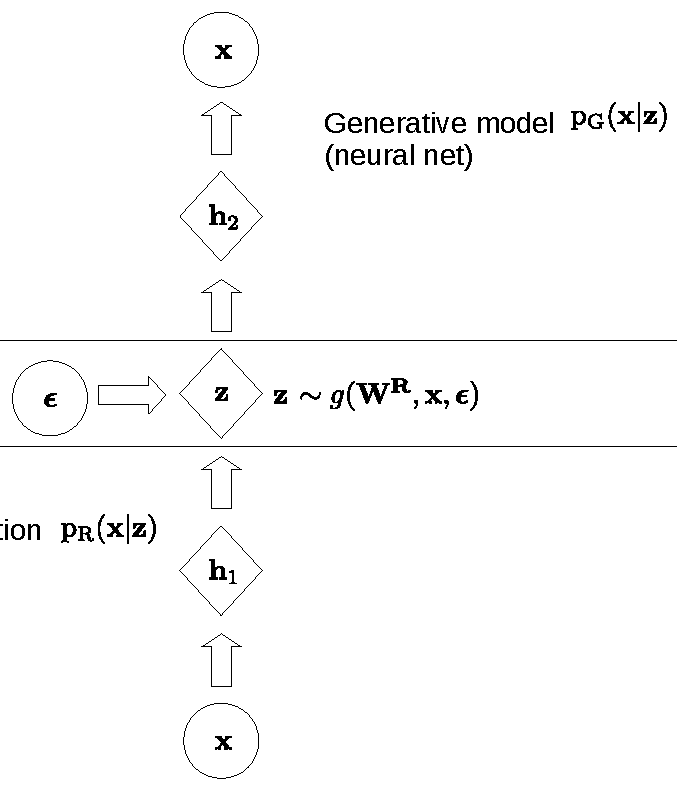
\includegraphics[width=.8\linewidth]{vae.pdf}
% %   \caption{Variational autoencoders...}
% %   \label{fig:vae}
% % \end{figure}
% 
% \paragraph{Solution: the reparametrization trick.}
% \begin{itemize}
% \item Choose $\epsilon \sim p_{\text{noise}}$ (noise distribution, independent of $\W^R$!)
% \item Set $\z = g(\W^{R}, \x, \epsilon)$, where $g$ is an appropriate class $\mathcal C^1$ function
%   \begin{itemize}
%   \item results in a sample $\z \sim p_R(.|\x)$, from the correct
%     posterior
%     \end{itemize}
% \end{itemize}
% The mapping $g$ should be taught of as a ``blurring'' function which produces noisy versions $\z$,
% called \textit{sensations}, of the true world state $\x$.
% The result is a scheme for training DBNs via good-old backprop!
% Refer to Fig. vae.pdf.
% % \ref{fig:vae}.
% Some examples of the reparametrization trick for a number of
% choices of the posterior distribution are given in Tab. \ref{tab:rptrick}.
% 
% \begin{table}[H]
%   \begin{tabular}{p{1.7cm}|p{1.5cm}|p{1.9cm}|p{2.1cm}|p{5cm}}
%          \hline
%          Posterior & $p_R(.|\x)$ & noise & $g(\W^R,\x,\epsilon)$ & Also \\ \hline
%          Normal & $\mathcal N(\mu,\sigma)$ & $\epsilon \sim \mathcal N(0, 1)$ & $\mu + \sigma \odot \epsilon$ & Location-scale family: Laplace, Elliptical,
%          Student’s t, Logistic, Uniform, Triangular, \ldots \\ \hline
%          Exponential & $\mathcal \exp(\lambda)$ & $\epsilon \sim \mathcal U([0, 1))$ & $-\log(1-\epsilon)/\lambda$ & Invertible CDF: Cauchy, Logistic, Rayleigh, Pareta, Weibull, Reciprocal, Gompert, Gumbel, Erlan, ... \\ \hline
%          Other & $\log\mathcal N(\mu,\sigma)$ & $\epsilon \sim \mathcal N(0, 1)$ & $\exp(\mu + \sigma \odot \epsilon)$ & Gamma, Dirichlet, Beta, Chi-squared, F, ... \\ \hline
%   \end{tabular}
%   \caption{Reparametrization trick \citep{kingma2013auto} for a variety of models.}
%   \label{tab:rptrick}
% \end{table}
% 
% For fixed $p_G(.|\x)$, the optimal choice for $p_R(.|\x)$ is given analytically by
% \begin{equation}
%   p_R(\z|\x) \propto p_G(\z|\x)\exp(-\Delta E_{G \rightarrow R}(\z, \x)).
% \end{equation}
% 
% \subsection{A thermodynamic model for bounded rationality, aka robust
%   optimality}
% \begin{itemize}
%   \item Recall that an agent is said to have \textit{bounded rationality} if they must take into account the cost of finding solutions to problems, and not just the utility of the final state.
%   \item For example, consider an agent that must operate under a limited lifetime and/or computation cost.
%   \item This is in contrast to agents with \textit{unbounded rationality} considered in classical game theory.
%     \end{itemize}
% The material presented is a revisit of \citep{braun2011path}. See also \citep{ortega2013thermodynamics}
% \paragraph{Utility functions and conjugate pairs.}
%   Let $(\Omega, \mathcal F, P)$ be a probablity space. A function $U: \mathcal F \rightarrow \mathbb R$ is said to be a \textit{utility function} for this space if the conditional utility $U(A|B) := U(A \cap B) - U(B)$ has the following propertites:
%   \begin{itemize}
%   \item additivity: $U(A_1 \cap A_2 | B) = U(A_1|B) + U(A_2|B)$, for all events $A_1, A_2, B \in \mathcal F$.
%   \item statistic: there exists a function $f_{U} :\mathbb R_+ \rightarrow \mathbb R$ such that $U(A|B) = f(P(A|B))$, for all events
%     $A,B \in \mathcal F$.
%   \item monotonicity: $f_{U}$ is strictly increasing.
%     \end{itemize}
% 
% \begin{theorem}
%   The only functions $f: \mathbb R_+ \rightarrow \mathbb R$ which is such that $U(A|B) \equiv f(P(A|B))$ any probability space $(\Omega, \mathcal F, P)$ and utility function $U$ thereupon are of the form
%   \begin{equation}
%     f = \alpha \log(.),
%     \label{eq:boltzmann}
%   \end{equation}
%   where $\alpha > 0$.
% \end{theorem}
% 
% \textbf{XXX: equation \eqref{eq:boltzmann} above looks like Boltzmann's formula (on his gravestone...)!}
% 
% Such $U$ and $P$ are said to form a \textit{conjugate pair} at temperature $\alpha$.
% 
% 
% \paragraph{Example.}
% Given a utility function $U$ on a probability space $(\Omega, \mathcal F, *)$, the \textit{Gibbs measure} at temperature $\alpha > 0$ and energy levels $(-U(\omega))_{\omega \in \Omega}$ is defined to be the probability measure (on thesame measurable space)
%   \begin{equation}
%     P(\omega) = \frac{1}{Z_{U}(\alpha)}\exp\left(\frac{1}{\alpha}U(\omega)\right), \; \forall \omega \in \Omega,
%   \end{equation}
%   where
% 
%   \begin{equation}
%     Z_{U}(\alpha) := \sum_{\omega \in \Omega}\exp\left(\frac{1}{\alpha}U(\omega)\right)
%   \end{equation}
%   is a normalization constant called the \textit{partition function} of $U$.
%   It's not hard to see that $U$ and the $P$ above form a conjugate pair.
% 
%   \paragraph{Free-utility functional.}
%     Let $(U, P)$ be a conjugate pair at temperature $\alpha > 0$  on a measurable space $(\Omega, \mathcal F)$. Given another probability measure $P'$ on the same space, define it's \textit{free utility} as
%     \begin{equation}
%       J(P'|U, P) = \langle U \rangle_{P'} + \alpha \mathcal H(P'),
%     \label{eq:free_u}
%     \end{equation}
%     where
%     \begin{equation}
%       \mathcal H(P') := \langle \log(P') \rangle_{P'} := -\sum_{\omega \in \Omega}P'(\omega)\log(P'(\omega))
%     \end{equation}
%     is the \textit{entropy} of $P'$ (measured in the Naperian base $e \approx 2.73$). It's not difficult to establish the upper bound
%   \begin{equation}
%     J(P'|U) \le J(P|U) = \sum_{\omega \in \Omega}U(\omega) =: U(\Omega).
%   \end{equation}
%   In particular, if $P$ is the Gibbs measure at temperature $\alpha$ corresponding to $U$, then the upper bound above reduces to the \textit{log-partition function}
%   \begin{equation}
%     J(P'|U) \le U(\Omega) = -\alpha \log(Z_{U}(\alpha)).
%     \end{equation}
% 
%   \paragraph{The free-energy / utility principle (of Friston ?).}
%   We are now in shape to introduce the notion of free-energy for model transitions, and a variational principle for optimizing it. Consider thus an initial system described by a conjugate pair $(U_{\text{ini}}, P_{\text{ini}})$ at temperature $\alpha > 0$. We want to transform this to a new model by adding constraints represented by the utility function $\Delta U$.  The resulting system has final utility $U_{\text{fin}} = U_{\text{ini}} + \Delta U$. The difference in free-utility is then
%   \begin{equation}
%     \Delta J_{(U_{\text{ini}}, P_{\text{ini}}) \rightarrow P_{\text{fin}}} := J_{\text{fin}} - J_{\text{ini}} = \underbrace{\langle \Delta U\rangle_{P_{\text{fin}}}}_{\textbf{accuracy}} -  \underbrace{\alpha D_{\text{KL}}(P_{\text{ini}}\|P_{\text{fin}})}_{\textbf{complexity}},
%     \label{eq:free}
%   \end{equation}
%   where
%   \begin{equation}
%     D_{\text{KL}}(P_{\text{fin}}\|P_{\text{ini}}) := \langle \log(\P_{\text{fin}}/\P_{\text{ini}})\rangle_{\P_{\text{fin}}} := \sum_{\omega \in \Omega}\P_{\text{fin}}(\omega)\log(\P_{\text{fin}}(\omega)/\P_{\text{ini}}(\omega))
%   \end{equation}
%   is the Kullback-Leibler divergence, and represents the information cost (measured in energy units) of changing the initial system.
% In the above formula, we've extensively used the fact that $(U_{\text{ini}}, P_{\text{ini}})$ is a congugate pair and so $U_{\text{ini}}(\omega) \equiv \alpha \log(P_{\text{ini}}(\omega))$ by virtue of \eqref{eq:boltzmann}.
%   The two terms in \eqref{eq:free} (accuracy or expected gain in utility, and the complexity of the transition) can be viewed as dertiminants of bounded rational decision-making. They formalize
% a trade-off between an expected utility $\Delta U$ (first term) and
% the information cost of transforming Pi
% into $P_{\text{fin}}$ (second
% term). In this interpretation $P_{\text{ini}}$ represents an initial choice
% probability or policy, which includes the special case of the
% uniform distribution where the decision-maker has initially no
% preferences between the different choices. The probability measure $P_{\text{fin}}$ is the final choice probability that we are looking for since it
% considers the utility constraint U∗
% that we want to optimize. We can then formulate a variational principle for bounded rationality in the probabilities $P_{\text{fin}}(\omega)$
% \begin{equation}
% P^*_{\text{fin}} := \underset{P_{\text{fin}}}{\text{argmax }} \Delta J_{(U_{\text{ini}}, P_{\text{ini}}) \rightarrow P_{\text{fin}}}
%   \end{equation}
% 
% By differentiating the RHS of \eqref{eq:free} w.r.t $P_{\text{fin}}$ and setting to zero, we obtain the closed-form solution
% 
% \begin{equation}
%   P^*_{\text{fin}}(\omega) \propto P_{\text{ini}}(\omega)\exp\left(\frac{1}{\alpha}\Delta U(\omega)\right).
% \end{equation}
% 
% Two limit cases are worth considering.
% \begin{itemize}
% \item \textbf{Low-temperature regime $\alpha \approx 0$:} Here $\Delta J_{(U_{\text{ini}}, P_{\text{ini}}) \rightarrow P_{\text{fin}}} \approx \langle \Delta U\rangle_{P'_{\text{fin}}}$, and so it's optimal to take
%   $$P^*_{\text{fin}}(\omega) \equiv \text{dirac}(\omega - \omega^*) = \begin{cases}1, &\mbox{if }\omega = \omega^*,\\0, &\mbox{ otherwise,}\end{cases}$$
%   where $\omega^* := \argmax_{\omega \in \Omega}U(\omega)$. This corresponds to unbounded rational decision-making, in which the cost of transition / problem-solving is completely disregarded.
%   \item \textbf{High-temperature regime $\alpha \rightarrow +\infty$:} In this limiting case, it's optimal to take $P^*_{\text{fin}}(\omega) \equiv P_{\text{ini}}(\omega)$, i.e the change is so costly that it's optimal to maintain the current choice probabilities.
% \end{itemize}
% 
% To conclude this section, let's note that \citep{braun2011path} show how their free-energy framework (on paths) links with the well-known Hamilton-Jacobi-Bellman optimal control framework. For example, one can re-derive the Linear Quadratic Gaussian (LQG) controller, which is a generalization of the LQR in \eqref{eq:hj}...
% 
% 
% \subsection{GANs and other likelihood-free methods}
% \ldots


\end{document}
